\documentclass[12pt,reqno, twoside]{amsbook}
%%%%%%%%%%%%%%%%%%%%%%%%%%%%%%%%%%%%%%%%%%%%%%%%%%%%%%%%%%%%%%%%%%%%%%%%%%%%%%%%%%%%%%%%%%%%%%%%%%%%%%%%%%%%%%%%%%%%%%%%%%%%%%%%%%%%%%%%%%%%%%%%%%%%%%%%%%%%%%%%%%%%%%%%%%%%%%%%%%%%%%%%%%%%%%%%%%%%%%%%%%%%%%%%%%%%%%%%%%%%%%%%%%%%%%%%%%%%%%%%%%%%%%%%%%%%
\usepackage{eurosym}
\usepackage{placeins}
\usepackage{amsmath}
\usepackage{amssymb}
\usepackage{amsfonts}
\usepackage[onehalfspacing]{setspace}
\usepackage{chngcntr}
\usepackage{graphicx}
\usepackage[a4paper, margin=2.5cm]{geometry}
\usepackage[english]{babel}
\usepackage{fancyhdr}
\usepackage{titlesec}
\usepackage{enumitem}
\usepackage{etoolbox}
\usepackage[backend=biber, style=ieee, sorting=none]{biblatex}
\addbibresource{bib/refs.bib}
\usepackage{url}           % for clickable URLs
\usepackage{hyperref}
\usepackage{enumitem}
\usepackage{acronym}
\usepackage{listings}
\usepackage{xcolor}
\usepackage{booktabs}
\usepackage{multirow}
\usepackage{adjustbox}
\usepackage{tikz}
\usetikzlibrary{shapes.geometric, arrows.meta, positioning}

\lstset{
    basicstyle=\ttfamily\small,
    breaklines=true,
    frame=single,
    backgroundcolor=\color{gray!5},
    captionpos=b,
    columns=fullflexible,
    keepspaces=true
}

% you may need to uncomment the command below if you use eps format for figures
%\usepackage{epstopdf}

% These packages are not part of the template made available by ISCTE
\usepackage{eurosym}
\usepackage{amsmath, amssymb, amsfonts}
\usepackage[onehalfspacing]{setspace}
\usepackage{chngcntr}
\usepackage{graphicx}
\usepackage[a4paper, margin=2.5cm]{geometry}
\usepackage[english]{babel}
\usepackage{fancyhdr}
\usepackage{titlesec}
\usepackage{enumitem}
\usepackage{etoolbox}
\usepackage{url}
\usepackage{hyperref}
\usepackage{xcolor}
\usepackage{acronym}
\usepackage{caption}
\usepackage{subcaption}

\numberwithin{figure}{chapter}
\numberwithin{table}{chapter}
\numberwithin{equation}{chapter}

\usepackage{xcolor}
%end of the extra packages

\makeatletter
    \def\section{\@startsection{section}{1}%
      \z@{.5\linespacing\@plus.7\linespacing}{.25\linespacing}%
      {\normalfont\bfseries\flushleft}}
    \def\subsection{\@startsection{subsection}{2}%
      \z@{.5\linespacing\@plus.7\linespacing}{.25\linespacing}%
      {\normalfont\bfseries\flushleft}}

\makeatother
\setcounter{MaxMatrixCols}{10}

\providecommand{\U}[1]{\protect\rule{.1in}{.1in}}
\theoremstyle{plain}
\newtheorem{acknowledgement}{Acknowledgement}
\newtheorem{algorithm}{Algorithm}[chapter]
\newtheorem{axiom}{Axiom}[chapter]
\newtheorem{case}{Case}[chapter]
\newtheorem{claim}{Claim}[chapter]
\newtheorem{conclusion}{Conclusion}[chapter]
\newtheorem{condition}{Condition}[chapter]
\newtheorem{conjecture}{Conjecture}[chapter]
\newtheorem{corollary}{Corollary}[chapter]
\newtheorem{criterion}{Criterion}[chapter]
\newtheorem{definition}{Definition}[chapter]
\newtheorem{example}{Example}[chapter]
\newtheorem{exercise}{Exercise}[chapter]
\newtheorem{lemma}{Lemma}[chapter]
\newtheorem{notation}{Notation}[chapter]
\newtheorem{problem}{Problem}[chapter]
\newtheorem{proposition}{Proposition}[chapter]
\newtheorem{remark}{Remark}[chapter]
\newtheorem{solution}{Solution}[chapter]
\newtheorem{summary}{Summary}[chapter]
\newtheorem{theorem}{Theorem}[chapter]
\numberwithin{equation}{chapter}


% Please write the references according to your school

\newenvironment{dedication}
  {%\clearpage           % we want a new page
   \thispagestyle{empty}% no header and footer
   \vspace*{\stretch{1}}% some space at the top
   \itshape             % the text is in italics
   \raggedleft          % flush to the right margin
  }
  {\par % end the paragraph
   \vspace{\stretch{3}} % space at bottom is three times that at the top
   %\clearpage           % finish off the page
  }
  \numberwithin{section}{chapter}
\fancyhead{}
\fancyfoot{}
\pagestyle{fancy}
\fancyfoot[LE,RO]{\thepage}

\makeatletter
\def\ps@plain{\ps@empty
 \def\@evenfoot{%
   \normalfont\scriptsize
   \rlap{\thepage}\hfil
   }%
 \def\@oddfoot{%
   \normalfont\scriptsize \hfil
   \llap{\thepage}}%
}
\makeatother
\renewcommand{\headrulewidth}{0pt}
\renewcommand{\footrulewidth}{0pt}






%%%%%%%%%%%%%%%%%%%%%%%%%%%%%%%%%%%%%%%%%%%%%%%%%%%%%%%%%%%%%%%%%%%%%%%%%%%%%%%%%%%%%%%%
% Cover that doesn't come with the template provided by ISCTE
% Overleaf says there are errors with this section, but it renders fine so just ignore them

\definecolor{coverline}{RGB}{66, 81, 160}
\def\hrulefill{\leavevmode\leaders\hrule height 2pt\hfill\kern\z}

\begin{document}

\sffamily
\begin{flushleft}

\includegraphics[width=6.03cm]{images/iscte}\\[3mm]
\begin{large}
{\fontfamily{Montserrat-TOsF}\selectfont

~\\
~\\
Pattern Detection in Energy Consumption\\
~\\
~\\
Gonçalo Rosa\
~\\
~\\
Master's in data science\\
~\\
~\\
~\\
Supervisor:\\
PhD Ana Maria de Almeida, Associate Professor,  \\
ISCTE, Departamento de Ciências e Tecnologias de Informação\\
~\\
Co-Supervisor:\\
PhD Diana Mendes, Associate Professor,\\
ISCTE, Departamento de Ciências e Tecnologias de Informação \\
~\\
~\\
~\\
September, 2025}
\end{large}
\end{flushleft}
\thispagestyle{empty}
\cleardoublepage
\begin{flushleft}
 % 
\includegraphics[width=6.03cm]{images/ista.png}\\[7mm]
 \begin{figure}[h]
  \centering
  \subfloat{
\includegraphics[width=.34\linewidth]{images/ista.png}}\hfill
  \subfloat {
\includegraphics[width=.34\linewidth]{images/ibs.png}}
\end{figure}
\begin{large}
{\fontfamily{Montserrat-TOsF}\selectfont

~\\
~\\
Department of Information Sciences and Technologies
~\\
Department of Quantitative Methods for Management and Economics
~\\
~\\
Pattern Detection in Energy Consumption\\
~\\
~\\
Gonçalo Rosa\\
~\\
~\\
Master's in Data Science\\
~\\
~\\
~\\
Supervisor:\\
PhD Ana Maria de Almeida, Associate Professor,  \\
ISCTE, Departamento de Ciências e Tecnologias de Informação\\
~\\
Co-Supervisor:\\
PhD Diana Mendes, Associate Professor,\\
ISCTE, Departamento de Ciências e Tecnologias de Informação \\
~\\
~\\
~\\
September 2025}
\end{large}
  \end{flushleft}
  \thispagestyle{empty}
\rmfamily
\normalsize
\frontmatter
\frontmatter
%\addtocontents{toc}{\setcounter{tocdepth}{2}}
\addtocontents{toc}{\setcounter{tocdepth}{2}}
\thispagestyle{empty}
\thispagestyle{empty}
\counterwithout{figure}{chapter}

\frontmatter
\addtocontents{toc}{\setcounter{tocdepth}{2}}
\thispagestyle{empty}
%%%%%%%%%%%%%%%%%%%%%%%%%%%%%%%%%%%%%%%%%%%%%%%%%%%%%%%%%%%%%%%%%%%%%%%%%%%%%%%%%%%%%%%%%%%%%%%%%%%%%%%%%%%%
\counterwithin{figure}{chapter}




%\begin{document}
\frontmatter
\addtocontents{toc}{\setcounter{tocdepth}{2}}
\thispagestyle{empty}

\begin{dedication}%

\begin{flushright}
\textit{To my family and friends,\\for their patience and encouragement.}
\end{flushright}%
\end{dedication}

\setcounter{page}{1}
\pagenumbering{roman} %
\chapter*{Acknowledgment}

I would like to express my sincere gratitude to my supervisors, PhD Ana Maria de Almeida and PhD Diana Mendes, for their guidance, constructive feedback, and continued support throughout the development of this dissertation.

I also wish to thank the GoiEner energy cooperative for making the smart meter dataset publicly available through Zenodo, enabling this and other data-driven studies of residential energy consumption.

\chapter*{Resumo}
A crescente utilização de \textit{smart meters} permite às empresas de energia recolher dados detalhados sobre o consumo de eletricidade ao longo do tempo. Embora estes dados ofereçam informações importantes sobre a forma como a energia é utilizada, apresentam frequentemente anomalias causadas por problemas técnicos, falhas de comunicação ou erros no processamento dos dados. Estas anomalias podem resultar em faturas incorretas, ineficiências operacionais e perda de confiança por parte dos consumidores.

Esta dissertação analisa a forma como padrões e anomalias podem ser identificados em dados de consumo energético provenientes de contadores inteligentes. É realizada uma revisão sistemática da literatura para compreender as abordagens atuais de deteção de anomalias, com especial enfoque em métodos não supervisionados, baseados em previsão e em clustering. Com base nessa revisão, é desenvolvida uma metodologia prática que inclui o pré-processamento dos dados, a análise da sazonalidade, tendência e estrutura residual ao nível da população, e a aplicação de um conjunto de algoritmos de deteção de anomalias sobre séries diárias de consumo agregado por município.

Os métodos são avaliados em três municípios do norte de Espanha pertencentes à cooperativa GoiEner, onde não existem dados de anomalias rotuladas. Os resultados mostram que uma abordagem de ensemble baseada em previsão, combinando N-BEATS com votação maioritária de cinco detetores, produz taxas de anomalia operacionalmente interpretáveis e identifica perturbações de consumo associadas a eventos reais, contribuindo para uma análise de dados mais fiável e uma melhor gestão energética.


\chapter*{Abstract}

The growing use of smart meters allows energy providers to collect detailed electricity consumption data over time. While this data offers important insights into how energy is used, it often contains anomalies caused by technical problems, communication failures, or data processing errors. These anomalies can result in incorrect bills, operational inefficiencies, and reduced trust from consumers.

This dissertation studies how patterns and anomalies can be identified in smart meter energy consumption data. A systematic review of existing research is carried out to understand current anomaly detection approaches, with a focus on unsupervised, prediction-based, and clustering methods. Based on this review, a practical methodology is developed that covers data preprocessing, population-level analysis of seasonal, trend, and residual structure, and the application of multiple anomaly detection algorithms to daily municipal aggregate consumption series.

The methods are evaluated across three municipalities in northern Spain from the GoiEner cooperative dataset, where no labeled anomaly ground truth is available. The results show that a prediction-based ensemble approach combining N-BEATS forecasting with majority-vote detection across five algorithms produces operationally practical anomaly rates and identifies consumption disruptions that correspond to real-world events, contributing to more reliable energy data analysis and improved operational monitoring.


\tableofcontents

%%%%%%%%%%%%%%%%%%%%%%%%%%%%%%%%%%%%%%%%%%%%%%%%%%%%%%%%%%%%%%%%%%%%%%%%%%%%%%%%%%%%%%%%%%%%%%%%%%%%%%%%%%%%%%%%%%%
% Also not in the original template
% Remove the ones you don't need
\listoffigures

\listoftables
\cleardoublepage

\chapter*{List of Acronyms}

\begin{acronym}[PRISMA]  
    \acro{CRISP-DM}{Cross-Industry Standard Process for Data Mining }
    \acro{IoT}{Internet of Things}
    \acro{AMI}{Advanced Metering Infrastructure}
    \acro{SLR}{Systematic Literature Review}
    \acro{STL}{Seasonal and Trend decomposition using Loess}
    \acro{PRISMA}{Preferred Reporting Items for Systematic Reviews and Meta-Analyses}
    \acro{AI}{Artificial Intelligence}
    \acro{ML}{Machine Learning}
    \acro{LSTM}{Long Short-Term Memory}
    \acro{CINN}{conditional Invertible Neural Networks}
    \acro{CVA}{conditional Variational Autoencoders}
    \acro{LOF}{Local Outlier Factor}
    \acro{SVM}{Support Vector Machine}
    \acro{PCA}{Principal Component Analysis}
    \acro{GMMs}{Gaussian Mixture Models}
    \acro{DR}{Demand Response}
    \acro{CNN}{Convolutional Neural Network}
    \acro{RNN}{Recurrent Neural Network}
    \acro{CV}{Coefficient of Variation}
    \acro{CNAE}{Clasificación Nacional de Actividades Económicas}
    \acro{MAE}{Mean Absolute Error}
    \acro{RMSE}{Root Mean Squared Error}
    \acro{MAPE}{Mean Absolute Percentage Error}
    \acro{sMAPE}{Symmetric Mean Absolute Percentage Error}
    \acro{pp}{percentage point}
    \acro{SARIMA}{Seasonal Autoregressive Integrated Moving Average}
    \acro{SARIMAX}{Seasonal Autoregressive Integrated Moving Average with eXogenous inputs}
    \acro{RF}{Random Forest}
    \acro{NBEATS}[N-BEATS]{Neural Basis Expansion Analysis for Time Series}
\end{acronym}
\acresetall

\cleardoublepage
%\printglossary[type=\acronymtype, nonumberlist, nogroupskip]

%%%%%%%%%%%%%%%%%%%%%%%%%%%%%%%%%%%%%%%%%%%%%%%%%%%%%%%%%%%%%%%%%%%%%%%%%%%%%%%%%%%%%%%%%%%%%%%%%%%%%%%%%%%%%%%%%%



\mainmatter



\hyphenation{wri-te he-re pro-per hy-phe-ni-za-tion}%

\setcounter{page}{1} \pagenumbering{arabic}



% =====================================================================
%                               MAIN BODY
% ====================================================================
\mainmatter
\hyphenation{wri-te he-re pro-per hy-phe-ni-za-tion}%
\setcounter{page}{1} \pagenumbering{arabic}


%%%%%%%%%%%%%%%%%%%%%%%%%%%%%%%%%%%%%%%%%%%%%%%%%%%%%%%%
\chapter{Introduction}
\label{chapter:intro}
%%%%%%%%%%%%%%%%%%%%%%%%%%%%%%%%%%%%%%%%%%%%%%%%%%%%%%%
%\noindent You must use $\backslash$noindent at the beginning of the first paragraph in sesctions and subsections.

%%%%%%%%%%%%%%%%%%%%%%%
%%%%%%%%%%%%%%%%%%%%%%%
\section{Context}
\label{section:context}
\noindent Energy costs have risen sharply in recent years, and getting billing right depends on having reliable consumption measurements. This dissertation looks at how patterns and anomalies can be identified in smart meter data, and how different algorithms compare at detecting both normal and abnormal consumption behaviour. Smart meters are now widely installed across energy markets, giving retailers and network operators access to large volumes of detailed data recorded as often as every 15 minutes. This level of detail makes it possible to track how households actually use energy — capturing daily habits, demand patterns, and how these shift over time \cite{hernandez_detection_2024}. Working at this granularity gives a much better basis for anomaly detection than relying on aggregated readings, which average out the variation that reveals problems \cite{himeur_artificial_2021}. That said, the same data also comes with reliability issues: irregular or faulty readings are common in real deployments and cannot simply be ignored.

These readings frequently show anomalies: abrupt spikes, unexpected drops, missing data, or persistent deviations from a customer's typical history. Such issues often stem from faulty sensors, communication failures, misconfigured hardware, or improper installations rather than actual changes in energy use. When these faults go unnoticed, they cause billing errors that frustrate overcharged customers or create financial losses through under-charging, while also forcing expensive manual inspections \cite{gaur_performance_2019}. Worse still, undetected anomalies can mask underlying equipment faults that may eventually become safety hazards \cite{himeur_artificial_2021}.

Simple rule-based detection is not enough to deal with data this complex. A more useful approach is to first learn what normal consumption looks like, and then flag readings that deviate from it. Smart meter data is well-suited for this: it captures detailed, continuous patterns that reflect real habits and routines. Research has shown that working at this resolution reveals structure and variation that disappears when data is aggregated \cite{hernandez_detection_2024}. Once a model has learned what typical consumption looks like for a given setting, irregular readings can be identified as genuine deviations rather than just statistical noise. Static thresholds and single baselines tend to miss this nuance \cite{gaur_performance_2019}.

In practice, many systems in the industry still rely on basic thresholds or manual checks that are only triggered after a customer raises a complaint. These approaches do not scale to millions of meters and cannot account for how much energy use naturally varies between people and seasons\cite{gaur_performance_2019}. Consumption is shaped by weather, time of day, and changing routines, which makes it genuinely hard to separate a real lifestyle change from a faulty reading. There is also no universal definition of what counts as an anomaly, and labelled examples of confirmed faults are rarely available.

There is still no clear consensus on the best way to flag anomalies across different types of energy consumers. Getting this right matters for billing accuracy, operational costs, and consumer trust. Any practical solution needs to handle high-frequency data\cite{mao_research_2024}, tolerate noisy measurements, and work without needing labelled fault examples\cite{m_z_h_unsupervised_2021}.

This dissertation tackles these challenges by studying how to reliably identify abnormal energy consumption patterns using a prediction-based approach. The idea is to model what normal consumption looks like, and then flag days where actual consumption deviates significantly from what was expected. Better detection means fewer billing errors, lower inspection costs, and a more proactive approach to managing the network.

\par

%%%%%%%%%%%%%%%%%%%%%%%
%%%%%%%%%%%%%%%%%%%%%%%
\section{Motivation}
\label{section:motivation}

\noindent In the energy market, consumption readings determine what customers are charged and form the basis for how retailers manage their networks. Keeping this data accurate and consistent matters for trust between consumers, retailers, and grid operators\cite{jan_global_2025, gaur_performance_2019}.

Problems arise when readings are wrong. Faulty meters, installation errors, communication failures, and data processing issues can all introduce anomalies that go unnoticed for long periods. When they do, the consequences show up in billing disputes, financial losses, and wasted time on manual investigations that could have been avoided\cite{gaur_performance_2019}.

Smart meters have changed what is possible here. Instead of a single monthly reading, operators now have hourly data for each customer — enough to see daily habits, weekly patterns, and how consumption changes across seasons. Aggregated data misses most of this variation and makes it harder to tell normal from abnormal behaviour \cite{himeur_artificial_2021}.

Pattern recognition methods fit naturally into this setting. By learning from historical data what typical consumption looks like, they can flag days where something unexpected happened — without needing a fixed threshold or a labelled example of a fault. Studies applying data-driven methods to energy time series have shown they capture structure that static approaches simply miss \cite{zangrando_anomaly_2022, benfer_semantic_2024}.

Detecting anomalies automatically and reliably is therefore a practical priority. It directly affects billing accuracy, cuts the cost of manual inspections, and helps operators catch technical faults before they escalate. High-resolution smart meter data makes this feasible; the challenge is building methods robust enough to tell apart genuine consumption changes from data errors and equipment faults.

This thesis approaches that challenge at the level of municipal aggregates, not individual meters. Individual smart meter series are too short and too noisy for reliable daily forecasting — on any given day a single user may be away from home, have a broken appliance, or just consume unusually, and those one-off events dominate the signal. Summing consumption across all active meters in a city produces a stable daily series where seasonal and trend structure is clear enough to model properly. Anomalies are then identified as days where that city-level total departs from what the model predicted. Detecting anomalies at the single-meter level (billing errors on individual accounts, faulty devices) is outside the scope of this framework. That trade-off is discussed in Chapter 5.

\par



\vspace{\baselineskip}


%%%%%%%%%%%%%%%%%%%%%%%
%%%%%%%%%%%%%%%%%%%%%%%
\section{Objectives and Research Questions} 
\label{section:objectives}
\noindent  Considering the challenges presented in the research,

\begin{enumerate}[leftmargin=1.5cm,label=RQ\arabic*:,itemsep=.5ex]
                 \item How are smart meter data readings structured?
              \item In what ways do the seasonality, tendency, and residual components behave?
                 \item What existing patterns of energy consumption are there?
                \item Which anomaly detection algorithms perform best?
\end{enumerate}

%%%%%%%%%%%%%%%%%%%%%%%
%%%%%%%%%%%%%%%%%%%%%%%
\section{Research Methodology}
\label{section:methodology}

This dissertation adopts the Cross-Industry Standard Process for Data Mining \ac{CRISP-DM} methodology \cite{wirth_crisp_2000} as the guiding framework for analyzing smart meter energy consumption data. CRISP-DM was chosen because it provides a clear, iterative structure for data-driven research while remaining flexible enough to accommodate the practical challenges of real-world datasets. This is particularly important for smart meter data, which is high-frequency, noisy, and lacks a universally accepted definition of what constitutes anomalous behavior.

The Business Understanding phase focuses on defining the problem addressed in this study: identifying abnormal energy consumption patterns in smart meter time-series data when labeled examples are limited or unavailable. This phase draws on a review of the literature on energy consumption patterns, analytics, and anomaly detection, which helps define the objectives of the study and the practical constraints the analysis needs to respect.

In the Data Understanding phase, the characteristics of the available smart meter dataset are examined in detail. This includes exploring consumption trends, seasonal patterns, data granularity, and data quality issues such as missing values or outliers. Insights gained at this stage guide later methodological decisions and help ensure that the chosen analytical techniques are appropriate for the data.

The Data Preparation phase involves transforming raw consumption readings into a form suitable for modeling. This includes cleaning and normalizing the data, handling missing or inconsistent values, and extracting features that capture meaningful usage behavior over time. Particular attention is given to preserving temporal structure and seasonal effects, which are critical for accurately identifying deviations in energy consumption.

During the modeling phase, unsupervised anomaly detection techniques are applied to the prepared data. Rather than proposing entirely new algorithms, this study focuses on adapting and combining established methods (clustering-based, density-based, and reconstruction-based) to evaluate their effectiveness on smart meter data. These models are trained to learn typical consumption patterns and to flag deviations that may indicate anomalous behavior.

The Evaluation phase assesses the performance and usefulness of the detected anomalies. Quantitative metrics are used where applicable, complemented by qualitative analysis to determine whether flagged patterns are meaningful and interpretable from an energy consumption perspective. Feedback from this stage may lead to adjustments in preprocessing or modeling, reflecting the iterative nature of CRISP-DM.

Finally, the Deployment phase is considered from a conceptual perspective. While full operational deployment is beyond the scope of this dissertation, the results are analyzed with practical implementation in mind, demonstrating how the proposed framework could be integrated into real-world energy monitoring or decision-support systems.

Structuring the methodology around CRISP-DM provides a transparent and repeatable workflow that bridges academic research and practical data analysis, with findings that are both methodologically sound and relevant to modern energy systems.

%%%%%%%%%%%%%%%%%%%%%%%%%%%%%%%%%%%%%%%%%%%%%%%%%%%%%%%%
\chapter{Literature Review}
\label{chapter:LitReview}
%%%%%%%%%%%%%%%%%%%%%%%%%%%%%%%%%%%%%%%%%%%%%%%%%%%%%%%%
\noindent
\ac{IoT} sensors, \ac{AMI}, and smart meters have made energy management far more data-intensive over the past decade. Today's meters record consumption at intervals as short as 15 to 60 minutes, producing a continuous stream of readings across residential, commercial, and industrial settings \cite{himeur_artificial_2021}. This wealth of data opens up new ways to detect unusual patterns — whether caused by equipment faults \cite{gaur_performance_2019}, sensor errors, changes in how people behave, operational problems \cite{turowski_enhancing_2022}, or deliberate actions like electricity theft \cite{liu_unsupervised_2024}.

Being able to spot these anomalies matters for demand forecasting, load balancing, consumer profiling, and the overall stability of the grid \cite{m_z_h_unsupervised_2021}. Yet the problem is genuinely difficult. Consumption patterns vary a great deal depending on weather, building type, and daily routines. And because confirmed fault examples are rarely labelled in real datasets, it is hard to train and validate detection models properly.

\par

%%%%%%%%%%%%%%%%%%%%%%%
%%%%%%%%%%%%%%%%%%%%%%%
\section{Systematic Literature Review}
\label{section:SLR}
A systematic literature review \ac{SLR} was conducted to investigate anomaly detection approaches applied to energy consumption time-series data, with particular emphasis on methods operating on smart meter and energy reading datasets. The review aimed to compare different learning paradigms, including unsupervised methods, supervised methods, and clustering-based approaches, as applied to temporal energy data.

The search strategy followed \ac{PRISMA} guidelines and was implemented using Scopus, semantic scholar and web of science. A structured search query was employed, combining three conceptual components:
\begin{enumerate}[label=(\roman*)]
    \item Energy-related data sources (``energy readings,'' ``energy consumption,'' ``smart meters,'' ``energy pattern recognition'')
    \item Temporal data representation (``time series,'' ``time readings'')
    \item Learning paradigms (``unsupervised methods,'' ``supervised methods,'' ``clustering'')
\end{enumerate}

\begin{table}[ht]
\centering
\caption{Pattern Recognition Search Strategy Components}
\label{tab:pattern_recognition_search_strategy}
\begin{adjustbox}{max width=\textwidth}
\begin{tabular}{lp{10cm}}
\hline
\textbf{Component} & \textbf{Keywords and Boolean Logic} \\ \hline
Data Sources & "energy reading*" OR "energy consumption" OR "smart meter*" OR "energy pattern recognition" \\
Representation & AND ("time series" OR "time reading*") \\
Paradigms & AND ("unsupervised" OR "supervised" OR "cluster*") \\
Number of Results & 180 \\ \hline
\textbf{Final String} & \texttt{TITLE-ABS-KEY( (C1) AND (C2) AND (C3) )} \\ \hline
\end{tabular}
\end{adjustbox}
\end{table}

\begin{enumerate}[label=(\roman*)]
    \item Energy-related data sources (``energy readings,'' ``energy consumption,'' ``smart meters,'' ``energy anomaly detection'')
    \item Temporal data representation (``time series,'' ``time readings'')
    \item Learning paradigms (``unsupervised methods,'' ``supervised methods,'' ``clustering'')
\end{enumerate}
\begin{table}[ht]
\centering
\caption{Anomaly Detection Search Strategy Components}
\label{tab:search_strategy}
\begin{adjustbox}{max width=\textwidth}
\begin{tabular}{lp{10cm}}
\hline
\textbf{Component} & \textbf{Keywords and Boolean Logic} \\ \hline
Data Sources & "energy reading*" OR "energy consumption" OR "smart meter*" OR "energy anomaly detection" \\
Representation & AND ("time series" OR "time reading*") \\
Paradigms & AND ("unsupervised" OR "supervised" OR "cluster*") \\
Number of Results & 165 \\ \hline
\textbf{Final String} & \texttt{TITLE-ABS-KEY( (C1) AND (C2) AND (C3) )} \\ \hline
\end{tabular}
\end{adjustbox}
\end{table}

\par
The combined search strategy was designed to capture a wide range of studies focused on anomaly detection in energy-related time-series data using various machine learning algorithms.

Across both search queries, a combined total of 345 publications were identified. After removing duplicates and screening titles and abstracts, I applied specific inclusion and exclusion criteria. This process narrowed the selection to peer-reviewed studies that focused specifically on energy or smart meter data, utilized explicit time-series analysis, and included an empirical evaluation of their detection methods. After a full-text review, 14 articles were chosen for an in-depth analysis \cite{brennan_prisma_2021}. Figure~\ref{fig:prisma} summarises the selection process.

\begin{figure}[htbp]
\centering
\begin{tikzpicture}[
    box/.style={rectangle, draw=black, thick, text width=7cm, minimum height=1.2cm, align=center, font=\small},
    sidebox/.style={rectangle, draw=black, thick, dashed, text width=5cm, minimum height=1.2cm, align=center, font=\small},
    arr/.style={->, >=Stealth, thick},
    node distance=1.6cm
]

\node[box] (id) {Records identified via Scopus, Semantic Scholar, and Web of Science \\ ($n = 345$: pattern recognition + anomaly detection searches)};

\node[box, below=of id] (screen) {Records after duplicate removal and title/abstract screening \\ ($n \approx 60$)};
\node[sidebox, right=1.5cm of screen] (excl1) {Records excluded \\ (duplicates, off-topic titles)};

\node[box, below=of screen] (elig) {Full-text articles assessed for eligibility \\ ($n \approx 30$)};
\node[sidebox, right=1.5cm of elig] (excl2) {Articles excluded \\ (no energy/smart meter data, \\ no empirical evaluation)};

\node[box, below=of elig] (incl) {Studies included in synthesis \\ ($n = 14$)};

\draw[arr] (id) -- (screen);
\draw[arr] (screen) -- (elig);
\draw[arr] (elig) -- (incl);
\draw[arr] (screen.east) -- (excl1.west);
\draw[arr] (elig.east) -- (excl2.west);

\end{tikzpicture}
\caption{PRISMA flow diagram for the systematic literature review. Intermediate counts marked $\approx$ are estimates; exact counts were not separately logged during screening.}
\label{fig:prisma}
\end{figure}

These selected studies cover several key domains, including building energy management systems, smart meter monitoring, and individual consumer energy profiling. Together, they represent the current state of research regarding anomaly detection techniques for energy time-series data.

The reviewed literature reveals a significant surge in research, fueled by the availability of high-resolution smart meter data and the growing need for automated analytics. There is a noticeable shift away from traditional statistical baselines toward more sophisticated hybrid models that combine deep learning, probabilistic modeling, and clustering. Several studies highlight core challenges in the field, such as the difficulty of working with unlabeled datasets \cite{gaur_performance_2019}, the need for models to be interpretable \cite{himeur_artificial_2021}, and the diverse, unpredictable nature of consumption behavior across different households and appliances \cite{zangrando_anomaly_2022}.

This \ac{SLR} forms the foundation for comparing algorithmic families and identifying methodological gaps addressed in this study.

%%%%%%%%%%%%%%%%%%%%%%%
%%%%%%%%%%%%%%%%%%%%%%%
\section{Discussion of Related Work} 
\label{section:relatedwork}

\noindent
\noindent
A growing body of research has explored how \ac{AI} and \ac{ML} can be used to detect anomalies in energy consumption data \cite{gaur_performance_2019}. The widespread adoption of smart meters has made large volumes of high-frequency data available, and there is increasing pressure to use it more effectively to reduce waste and improve grid management \cite{yan_intelligent_2024}.

Anomaly detection in this field is typically framed as finding patterns that deviate from what is considered normal \cite{m_z_h_unsupervised_2021}. The main difficulty is that normal behaviour varies widely across users and contexts, and confirmed examples of faults or errors are rarely available to train models on \cite{gaur_performance_2019}.

\subsection{Prediction-Based and Reconstruction-Based Approaches}

Prediction-based anomaly detection relies on forecasting models to establish a baseline for "normal" behavior, flagging any significant deviations between the predicted and actual values as anomalies. Transformer-based architectures and deep sequence models have gained traction here because they excel at capturing complex temporal patterns. For instance, Zhang et al. \cite{zhang_power_2021} integrated a Transformer forecasting model with K-Means clustering to categorize anomalous residuals, a method that outperformed traditional \ac{LSTM} baselines in hourly energy datasets. Similarly, Mao et al. \cite{mao_research_2024} introduced the AF-GS-Random-Forest framework, which uses autoformer predictions and a Random Forest classifier to analyze residuals, yielding notable gains in precision, recall, and F1-scores.

Reconstruction-based methods extend this by operating on latent-space representations rather than direct forecasting. Turowski et al. \cite{turowski_enhancing_2022} used conditional Invertible Neural Networks \ac{CINN} and conditional Variational Autoencoders \ac{CVA} to map raw load curves into a latent space where anomalies become more distinct. Both supervised and unsupervised detection models performed significantly better in this transformed space, suggesting that representation quality acts as an upstream bottleneck for detection accuracy.

While prediction and reconstruction models achieve competitive accuracy on large benchmarks, they require large-scale datasets, careful hyperparameter tuning, and substantial computational resources \cite{himeur_artificial_2021}.

\subsection{Unsupervised Machine Learning and Clustering-Based Algorithms}

Unsupervised techniques are the natural choice for anomaly detection in energy data, since real-world datasets rarely include labelled examples of faults. Clustering and density-based algorithms can identify outliers purely from the structure of the data, with no need for pre-labelled examples.

Zangrando et al. \cite{zangrando_anomaly_2022} performed one of the most thorough comparisons in the field, testing 12 different algorithms across 144 configurations on appliance-level data. Their findings revealed that classical machine learning models—specifically Isolation Forest \cite{liu_isolation_2008}, Local Outlier Factor \ac{LOF} \cite{breunig_lof_2000}, and One-Class \ac{SVM}—actually performed better than complex deep autoencoders. These traditional models also proved more flexible, generalizing well even when applied to appliances they weren't specifically trained on. Similarly, Jesmeen et al. \cite{m_z_h_unsupervised_2021} explored unsupervised clustering in smart homes, finding that \ac{LOF} consistently ranked among the best-performing methods once the data was refined through feature extraction and \ac{PCA}-based dimensionality reduction.

Other clustering frameworks, like Gaussian Mixture Models \ac{GMMs}, have also proven effective. Liu et al. \cite{liu_unsupervised_2024} introduced a multi-cluster feature selection method paired with a \ac{GMMs} classifier, which significantly improved the detection of abnormal user behavior and electricity theft. Meanwhile, Alonso et al. \cite{alonso_hierarchical_2020} advanced the field by developing hierarchical clustering algorithms based on quantile autocovariances. Their method allows for the efficient and robust grouping of load profiles on a massive scale.

These properties motivate the selection of Isolation Forest, \ac{LOF}, and One-Class \ac{SVM} in the detection pipeline described in Chapter~4.


\subsection{Statistical, Classical Machine Learning, and Hybrid Methods}

A large portion of existing research utilizes statistical and machine-learning techniques that rely on feature engineering and behavioral analysis to spot irregularities. Early methods often focused on regression-based baselines and daily anomaly scoring. For instance, Zhang et al. improved Demand Response \ac{DR} predictions by identifying and filtering out abnormal daily load patterns from historical data, ensuring more accurate forecasting \cite{zhang_anomaly_2011}.

As the field has progressed, researchers have shifted toward classical and deep learning models for analyzing smart meter data. Hernández et al. conducted a comparative study using random forests, decision trees, convolutional neural networks \ac{CNN}, and recurrent neural networks \ac{RNN} to detect anomalies in daily household routines \cite{hernandez_detection_2024}. Their findings showed that \ac{RNN} reached an F1-score of 0.8, proving particularly effective at spotting short-term behavioral shifts. In a similar vein, Leong et al. demonstrated how Fuzzy C-Means clustering can successfully identify abnormal human activity patterns by looking indirectly at energy usage spikes and dips \cite{leong_detection_2016}.

To handle the sheer volume of data produced by modern grids, hybrid frameworks combining machine learning with big data infrastructure have become more common. Yan et al. developed a system that merges large-scale data preprocessing with deep learning, showing strong results for real-time operational monitoring \cite{yan_intelligent_2024}.

Traditional statistical methods remain valued for interpretability and low computational cost, but machine learning and deep learning have become the preferred choice for handling the complex, nonlinear nature of modern energy consumption.

\subsection{Broader Perspectives and Review Studies}

Several review papers offer a high-level look at how this field has evolved. Himeur et al. provide one of the most detailed classifications of \ac{AI}-driven anomaly detection in energy, pinpointing major hurdles like the lack of labeled data, inconsistent ways of measuring success, privacy issues, and the difficulty of reproducing results across different studies \cite{himeur_artificial_2021}. Gaur et al. similarly highlight the need for standardized testing protocols and suggest using automated tools to create ground-truth labels so that findings can be compared across studies \cite{gaur_performance_2019}.

Other research focuses more on the patterns of energy use itself rather than just the errors. For instance, Rwegasira et al. look at consumption behavior, noting how time-based dynamics, missing data points, and operational changes create a heterogeneous and unstable signal environment that constrains model design \cite{rwegasira_time_2025}.

Taken together, these broad reviews highlight systemic problems (scarce labeled data, fragmented methodologies, inconsistent benchmarks) that make comparative studies like this dissertation necessary \cite{himeur_artificial_2021,gaur_performance_2019}.
%%%%%%%%%%%%%%%%%%%%%%%
\subsection{Summary}
\label{subsection:summary}

\noindent Prediction-, reconstruction-, and unsupervised learning–based approaches dominate anomaly detection research in energy systems, primarily due to the high dimensionality of consumption data and the lack of ground truth labeled anomalies. Prediction-based methods detect abnormal behavior through forecasting residuals, with recent Transformer-based models consistently outperforming traditional \ac{LSTM} architectures \cite{zhang_power_2021, mao_research_2024}. Reconstruction-based techniques further enhance detection by creating latent spaces where anomalies become more separable, as demonstrated with conditional \ac{CINN} and \ac{CVA} models \cite{turowski_enhancing_2022}. However, these methods typically require large datasets and substantial computational resources \cite{himeur_artificial_2021}.

Unsupervised algorithms remain a practical and effective alternative, particularly in real-world settings. Classical methods such as Isolation Forest, \ac{LOF}, and One-Class \ac{SVM} frequently outperform deep autoencoders while offering superior generalization and scalability \cite{zangrando_anomaly_2022, m_z_h_unsupervised_2021}. Clustering-based extensions, including \ac{GMMs} and hierarchical approaches, further facilitate large-scale deployment \cite{liu_unsupervised_2024, alonso_hierarchical_2020}. Statistical and classical machine learning techniques continue to be valued for their interpretability and computational efficiency, while hybrid frameworks increasingly integrate machine learning with big data infrastructures to meet real-time operational requirements \cite{zhang_anomaly_2011, hernandez_detection_2024, leong_detection_2016, yan_intelligent_2024}. Finally, existing review studies highlight persistent challenges, including limited labeled data, inconsistent evaluation practices, and reproducibility issues, underscoring the need for systematic and comparative analyses in this domain \cite{himeur_artificial_2021, gaur_performance_2019, rwegasira_time_2025}.




%%%%%%%%%%%%%%%%%%%%%%%%%%%%%%%%%%%%%%%%%%%%%%%%%%%%%%%%
\chapter{Methodology}
\label{chapter:Methodology}
\section{Dataset}
\subsection{Dataset description}
\label{subsection:Dataset}

\noindent Studying energy consumption patterns requires a dataset that covers a broad range of users over a long enough period to capture seasonal and behavioural variation. For this purpose, the \textit{GoiEner smart meters dataset} \cite{goiener_smart_meters_2022} was selected. It contains anonymized hourly electricity consumption readings from smart meters managed by the GoiEner energy cooperative in Spain, covering the period from 2014 to 2022.

The eight-year span and hourly resolution make it possible to examine the structure of smart meter readings in detail (RQ1) and to study seasonal, trend, and residual components over time (RQ2). The variety of consumption profiles across users supports the identification of recurring patterns (RQ3), and the presence of real-world data quality issues (missing values and unusual readings) makes the dataset a realistic setting for evaluating anomaly detection methods (RQ4).

\subsection{Dataset Structure and File Composition}
\label{subsection:Dataset Structure and File Composition}

\noindent
The GoiEner smart meters dataset is setup into multiple files that reflect different stages of data processing and distinct time periods. Each file contains anonymized user hourly electricity consumption time series associated with individual smart meters. The time series are uniformly indexed by timestamp and represent energy consumption measured in kilowatt-hours (kWh), allowing them to be treated as continuous temporal sequences.

The dataset includes both raw and processed versions of the time series. The \textit{raw} data files contain the original smart meter readings as collected from the metering infrastructure. These series may include missing values, irregular gaps, and measurement inconsistencies, reflecting the challenges typically encountered in real-world smart meter deployments. As such, the raw files are particularly useful for assessing data quality, understanding missing data patterns, and motivating preprocessing and anomaly detection strategies.

\noindent
In addition to the raw data, the dataset provides three imputed subsets corresponding to distinct temporal periods. These files contain time series in which missing values have been filled using a predefined imputation strategy, and an additional indicator is included to distinguish original observations from imputed values. The imputed datasets are segmented into pre-, during-, and post-COVID-19 time periods, reflecting different phases of societal and behavioral conditions.

For analytical convenience, a unified imputed dataset was constructed by concatenating the three imputed subsets into a single continuous time series for each smart meter. This merged file preserves the imputation indicators and temporal ordering of the original subsets, resulting in longer and more complete time series. The unified representation simplifies downstream tasks such as time-series decomposition, forecasting, and prediction-based anomaly detection, which benefit from extended and continuous temporal coverage.

Across all time-series files, each individual record follows a common structure consisting of a timestamp and a corresponding hourly consumption value. In the imputed files, an additional binary flag indicates whether the observation was imputed. This consistent structure enables comparative analysis between raw and processed data, supports time-series decomposition, and facilitates the application of unsupervised anomaly detection algorithms.
\noindent

\begin{table}[h]
\centering
\caption{Summary of dataset files and their main characteristics}
\label{tab:dataset_files}
\begin{adjustbox}{max width=\textwidth}
\begin{tabular}{llll}
\hline
\textbf{File} & \textbf{Time Period Covered} & \textbf{Data Status} \\
\hline
raw & 2014--2022 & Not imputed &  \\
imp-pre & Before March 2020 & Imputed \\
imp-in & March 2020 -- May 2021 & Imputed \\
imp-post & After May 2021 & Imputed \\
merged-imp & 2014--2022 & Imputed  \\

\hline
\end{tabular}
\end{adjustbox}
\end{table}

\noindent
\noindent
The merged imputed dataset consolidates all available temporal segments (pre-, during-, and post-periods) for each user into a single time series. As segment availability varies across users, the merged dataset does not enforce complete coverage of all periods but instead preserves all existing observations while explicitly marking segment presence. This representation enables modeling tasks that benefit from extended temporal continuity, such as forecasting and reconstruction-based anomaly detection, while the original segmented files are retained for analyses requiring strict period-specific comparisons.
\subsection{Metadata Description}
\noindent
In addition to the time-series consumption files, the dataset includes a metadata file that provides descriptive and contextual information for each smart meter time series. This metadata is essential for understanding the composition, duration, and quality of the data, as well as for filtering and grouping time series during analysis. Each row in the metadata file corresponds to a unique anonymized user identifier and summarizes key characteristics of the associated consumption series.
\begin{table}[h]
\centering
\caption{Description of the metadata file columns}
\begin{adjustbox}{max width=\textwidth}
\begin{tabular}{ll}
\hline
\textbf{Column} & \textbf{Description} \\
\hline
user & Anonymized identifier of the smart meter customer \\
start\_date & Timestamp of the first recorded observation \\
end\_date & Timestamp of the last recorded observation \\
length\_days & Total duration of the time series in days \\
length\_years & Total duration of the time series in years \\
potential\_samples & Expected number of hourly samples for the period \\
actual\_samples & Number of recorded hourly observations \\
missing\_samples\_abs & Absolute number of missing samples \\
missing\_samples\_pct & Percentage of missing samples \\
contract\_start\_date & Start date of the energy supply contract \\
contract\_end\_date & End date of the energy supply contract \\
contracted\_tariff & Tariff category associated with the contract \\
self\_consumption\_type & Type of self-consumption, if applicable \\
p1--p6 & Contracted power levels for tariff periods \\
province & Province of the consumer (coarse-grained) \\
municipality & Municipality of the consumer (coarse-grained) \\
zip\_code & Anonymized postal code \\
cnae & Economic activity classification code \\
\hline
\end{tabular}
\end{adjustbox}
\end{table}
\FloatBarrier
%%%%%%%%%%%%%%%%%%%%%%%%%%%%%%%%%%%%%%%%%%%%%%%%%%%%%%%%

\section{Data Understanding}
\subsection{Structure Analysis}

\noindent 
The dataset in this case contains records for 25559 users, however, not all of them are suitable for the purposes of our case study.
From the original metadata population, only 19,998 users had successfully generated merged imputed time series and were retained for subsequent modeling and seasonality analyses.
Therefore is necessary to assess whether the available data for each user exhibits an adequate composition and quality. To support this assessment, we leverage the percentage of missing samples associated with each time series. This metric allows us to identify users whose data contain substantial gaps and to analyze the overall distribution of missing values across the dataset.

Table \ref{tab:missing_distribution} summarizes the distribution of missing data percentages across all users. The results indicate that an overwhelming majority of users exhibit less than 5\% missing samples. Consequently, users with more than 5\% missing data can be safely excluded from the analysis without significantly affecting the representativeness of the dataset.

After applying this filtering criterion, the resulting dataset comprises 19,709 users. In the following step, we analyze how these users are distributed according to their electricity consumption profiles, with particular emphasis on the number of active tariff periods associated with each user.
\begin{table}[h]
\centering
\caption{Distribution of missing samples across users}
\label{tab:missing_distribution}
\begin{adjustbox}{max width=\textwidth}
\begin{tabular}{lrr}
\hline
\textbf{Missing samples range} & \textbf{Count} & \textbf{Percentage (\%)} \\
\hline
0--5\%   & 19\,709 & 98.55 \\
5--10\%  &    123  &  0.62 \\
10--15\% &     46  &  0.23 \\
15--20\% &     23  &  0.12 \\
20--25\% &     22  &  0.11 \\
25--30\% &     12  &  0.06 \\
30--35\% &     12  &  0.06 \\
35--40\% &      9  &  0.05 \\
40--45\% &      8  &  0.04 \\
45--50\% &      7  &  0.04 \\
50--55\% &      4  &  0.02 \\
55--60\% &      5  &  0.03 \\
60--65\% &      2  &  0.01 \\
65--70\% &      7  &  0.04 \\
70--75\% &      2  &  0.01 \\
75--80\% &      1  &  0.01 \\
80--85\% &      0  &  0.00 \\
85--90\% &      0  &  0.00 \\
90--95\% &      4  &  0.02 \\
95--100\%&      2  &  0.01 \\
\hline
\end{tabular}
\end{adjustbox}
\end{table}
\FloatBarrier

\noindent
An analysis of tariff profile distributions in figure\ref{fig:tariff_distribution} revealed that the majority of users (approximately 89\%) are associated with two active tariff periods. Consequently, this group was selected as the primary focus for subsequent analyses. Users with one or six active tariff periods were retained for comparative evaluation, while groups with zero or three active periods were excluded due to insufficient size or incomplete tariff information. Making the total users that are eligible to study being 19,709.

\begin{figure}[htbp]
    \centering
    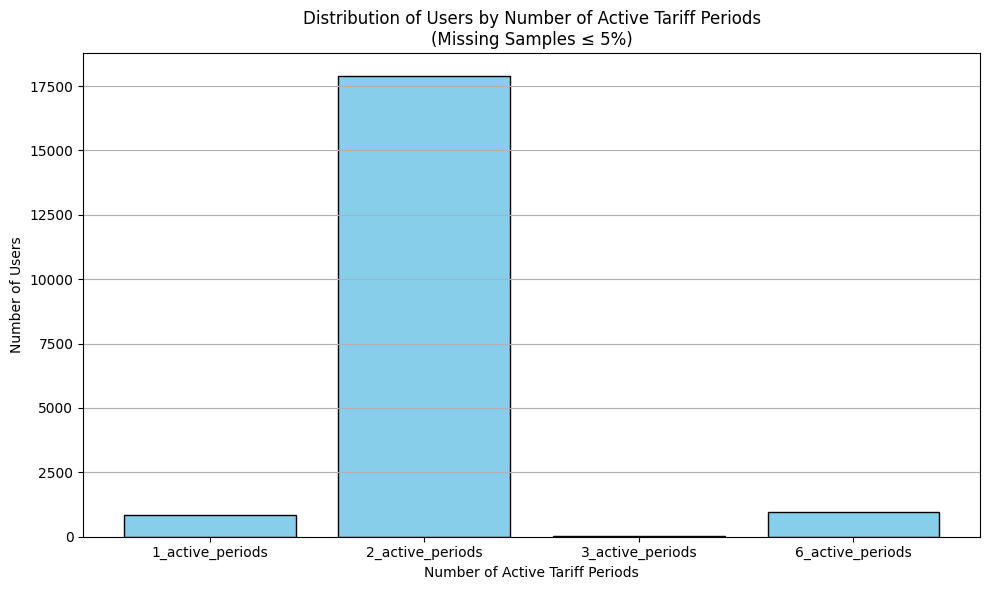
\includegraphics[width=1\textwidth]{images/distributionActiveTariffPeriods.png}
    \caption{Distribution of active tariff periods across the dataset.}
    \label{fig:tariff_distribution}
\end{figure}

 Having identified the most representative user profiles, the next logical step is to examine the temporal depth of the data. Record duration (years of data per user) is a critical factor for the stability of the time-series analysis. To visualize how this duration varies across the dataset, we employ a box-and-whisker plot, as shown in Figure \ref{fig:whiskerplot-lengthYearsByActivePeriods}.
 
\begin{figure}[htbp]
    \centering
    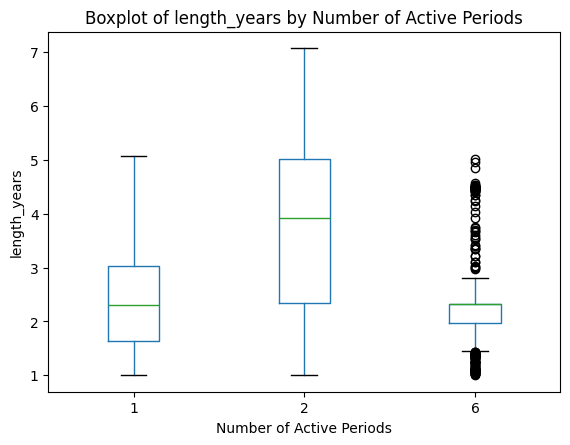
\includegraphics[width=0.7\textwidth]{images/whiskerplotoflengthyears.png}
    \caption{Distribution of length years by number of  active periods.}
    \label{fig:whiskerplot-lengthYearsByActivePeriods}
\end{figure}

Users with two active tariff periods exhibit significantly longer monitoring horizons, with a median duration exceeding three years and coverage extending up to seven years. Users with one or six active periods show shorter and more heterogeneous time-series lengths. Based on both group size and temporal coverage, the two-active-period group was selected as the primary population for subsequent analyses, while the remaining groups were retained for comparative evaluation.

Outliers are observed primarily in the six-active-period group, indicating greater heterogeneity in time-series duration within this profile. The one- and two-active-period groups show more compact distributions, with no values exceeding the interquartile range thresholds. This further supports the selection of the two-active-period group as the primary focus for analysis.

\begin{table}[h]
\centering
\caption{Distribution of contracted tariff period configurations}
\label{tab:tariff_fixtures}
\begin{adjustbox}{max width=\textwidth}
\begin{tabular}{lccc}
\hline
Tariff fixture (p1--p6) & Active periods & Users & Percentage (\%) \\
\hline
1-1-0-0-0-0 & p1, p2 & 17{,}870 & 90.81 \\
1-1-1-1-1-1 & p1--p6 &    939  &  4.77 \\
1-0-0-0-0-0 & p1     &    855  &  4.34 \\
1-0-1-0-0-0 & p1, p3 &     15  &  0.08 \\
\hline
\end{tabular}
\end{adjustbox}
\end{table}

Table \ref{tab:tariff_fixtures} reports the distribution of contracted tariff period configurations across the filtered user population, expressed in terms of absolute counts and relative percentages. Each configuration corresponds to a binary representation of the active tariff periods (p1–p6), derived from the contracted power metadata.
\par
The results reveal a highly skewed distribution of tariff configurations. The most common fixture, corresponding to users with active contracted power in periods p1 and p2, accounts for 90.81\% of the total population. This configuration reflects the dominant residential tariff structure within the dataset and aligns with the prevalence of users exhibiting two active tariff periods. Single-period configurations, represented by activity in p1 only, comprise 4.34\% of users, while users with all six tariff periods active represent 4.77\% of the population. Other configurations occur only marginally and account for a negligible proportion of users.
\par
Given the overwhelming dominance of the two-period configuration, subsequent analyses will mainly focus on this group to ensure statistical robustness and interpretability of results. Less frequent configurations are retained for comparative analysis where appropriate but are not used as the primary basis for pattern discovery or anomaly detection due to their limited representation.

\begin{table}[htbp]
\centering
\caption{Sample distribution by sector}
\label{tab:sector_distribution}
\small
\begin{adjustbox}{max width=\textwidth}
\begin{tabular}{clrr}
\toprule
\textbf{Rank} & \textbf{Sector} & \textbf{N} & \textbf{\%} \\
\midrule
1  & Household production                  & 16{,}311 & 80.7 \\
2  & Public administration                 &    612   &  3.0 \\
3  & Warehousing and logistics             &    481   &  2.4 \\
4  & Retail trade                          &    346   &  1.7 \\
5  & Education                             &    211   &  1.0 \\
6  & Food and beverage services            &    210   &  1.0 \\
7  & Associations                          &    171   &  0.8 \\
8  & Sports and recreation                 &    126   &  0.6 \\
9  & Construction (buildings)              &     89   &  0.4 \\
10 & Personal services                     &     82   &  0.4 \\
11 & Other professional services           &     80   &  0.4 \\
12 & Wholesale trade                       &     72   &  0.4 \\
13 & Agriculture, livestock, fishing       &     71   &  0.4 \\
14 & Water supply                          &     53   &  0.3 \\
15 & Accommodation                         &     45   &  0.2 \\
16 & Real estate                           &     45   &  0.2 \\
17 & Healthcare                            &     44   &  0.2 \\
18 & Specialized construction              &     37   &  0.2 \\
19 & Vehicle trade and repair              &     36   &  0.2 \\
20 & Social work                           &     33   &  0.2 \\
21 & Travel agencies                       &     31   &  0.2 \\
22 & Food manufacturing                    &     30   &  0.1 \\
23 & Legal and accounting                  &     30   &  0.1 \\
24 & Other manufacturing                   &     29   &  0.1 \\
25 & Metal products                        &     28   &  0.1 \\
26 & Unknown                               &     22   &  0.1 \\
27 & Office support                        &     20   &  0.1 \\
28 & Libraries, museums                    &     19   &  0.1 \\
29 & Architecture and engineering          &     18   &  0.1 \\
30 & Financial services                    &     18   &  0.1 \\
31 & Creative arts                         &     16   &  0.1 \\
32 & IT and programming                    &     16   &  0.1 \\
33 & Telecommunications                    &     16   &  0.1 \\
34 & Film, video, TV                       &     15   &  0.1 \\
35 & Printing and reproduction             &     15   &  0.1 \\
36 & Wood and cork                         &     15   &  0.1 \\
37 & Advertising                           &     13   &  0.1 \\
38 & Machinery                             &     11   &  0.1 \\
39 & Residential care                      &     10   & $<$0.1 \\
40 & Energy (electricity, gas)             &      8   & $<$0.1 \\
41 & Others (37 sectors)                   &    144   &  0.7 \\

   & \textbf{Total}                        & \textbf{20{,}222} & \textbf{100.0} \\
\bottomrule
\end{tabular}
\end{adjustbox}
\end{table}

The distribution of users across \ac{CNAE} sectors is highly uneven, with a strong concentration in a small number of categories. As shown in Table~\ref{tab:sector_distribution}, the majority of users belong to the Household production sector, which accounts for 16,311 users and dominates the dataset.

All other sectors are significantly smaller in comparison. The second largest group, Public administration, includes only 612 users, followed by Warehousing and logistics (481 users) and Retail trade (346 users). Beyond these categories, most sectors contain relatively few users, with many represented by only a handful of observations.

This distribution indicates a highly imbalanced dataset, where residential consumption patterns dominate the analysis. Consequently, aggregate results are likely to be strongly influenced by household behavior, while sector-specific patterns in smaller categories may be underrepresented.

At the same time, the presence of multiple smaller sectors provides an opportunity to explore heterogeneity in consumption behavior across different economic activities, however, the sample size of smaller sectors is too limited to draw meaningful conclusions.
\section{Seasonality Analysis}

\noindent Electricity consumption is inherently periodic. Daily routines, work schedules, and appliance usage impose recurring intraday fluctuations. Understanding this periodicity serves two purposes in this study: it characterises how regular or irregular different user groups are, and it provides the deterministic baseline that is later separated from irregular residuals in the anomaly detection pipeline \cite{m_z_h_unsupervised_2021, zangrando_anomaly_2022}.

\subsection{Decomposition Methodology}

Each user's merged hourly time series is decomposed into trend, seasonal, and remainder components using \ac{STL} \cite{cleveland_stl_1990}:
\begin{equation}
    x_t = T_t + S_t + R_t
    \label{eq:stl}
\end{equation}
where $T_t$ captures the long-term drift, $S_t$ the periodic pattern, and $R_t$ the irregular residual. Seasonal strength $F_s$ is then computed as:
\begin{equation}
    F_s = \max\!\left(0,\; 1 - \frac{\operatorname{Var}(R_t)}{\operatorname{Var}(S_t + R_t)}\right)
    \label{eq:seasonal_strength}
\end{equation}

A value near 1 means the seasonal component explains most of the variation once the trend is removed; a value near 0 indicates little periodic structure. The decomposition is applied at the daily frequency (period~=~24~h), independently for the three COVID temporal segments: pre (before March 2020), in (March 2020--May 2021), and post (after May 2021). While weekly periodicity (period~=~168~h) is not formally decomposed here, the weekday--weekend cycle is captured explicitly in the forecasting models through calendar features ($\sin$/$\cos$ day-of-week encoding and an \texttt{is\_weekend} binary flag), which are detailed in Section~\ref{sec:forecasting}. Weekly seasonal strength distributions were computed alongside the daily analysis but are not separately plotted; the calendar encoding in the forecasting pipeline is the primary mechanism for capturing the weekday--weekend pattern, and the STL-based weekly metric added no further analytical insight beyond what the daily decomposition already shows.

\subsection{Aggregate Daily Seasonality}

Figure~\ref{fig:daily_seasonality} shows the distribution of daily seasonal strength across all users in each period. The in-period exhibits the highest median ($F_s = 0.494$), followed by pre ($0.462$) and post ($0.452$), indicating that consumption patterns became more structured during the COVID-19 lockdowns and relaxed afterward. This is consistent with the broader finding that social disruptions such as mobility restrictions tend to homogenise daily routines and thereby strengthen periodic consumption signals \cite{rwegasira_time_2025}.

\begin{figure}[htbp]
    \centering
    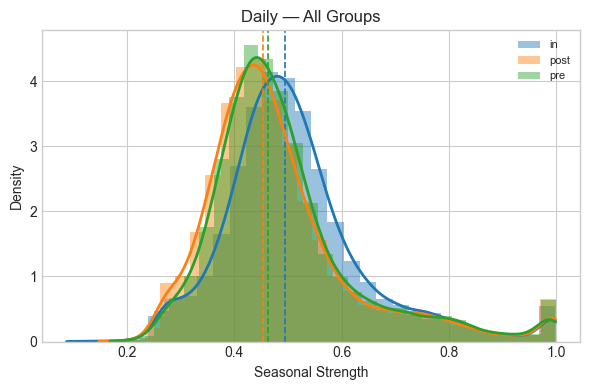
\includegraphics[width=\textwidth]{images/Daily_Seasonality.png}
    \caption{Distribution of daily seasonal strength ($F_s$) across all users for the pre-, in-, and post-COVID periods. The in-period distribution shifts visibly to the right, reflecting more structured daily routines during lockdown.}
    \label{fig:daily_seasonality}
\end{figure}

The aggregate distributions are positively skewed, with most users clustering around moderate seasonal strength while a smaller group exhibits highly regular behaviour. However, this aggregate view masks important sector-level differences, which are detailed in the sector-stratified analysis below (Table~\ref{tab:seasonality_comparison}).

\begin{table}[htbp]
\centering
\caption{Daily seasonal strength ($F_s$) by sector and COVID period}
\label{tab:seasonality_comparison}
\begin{adjustbox}{max width=\textwidth}
\begin{tabular}{llccccc}
\toprule
\textbf{Sector} & \textbf{Period} & \textbf{Mean} & \textbf{Median} & \textbf{Std} & \textbf{P25--P75} & \textbf{Skew} \\
\midrule
Household prod. & Pre  & 0.476 & 0.457 & 0.113 & 0.406--0.519 & $+$1.42 \\
Household prod. & In   & 0.501 & 0.489 & 0.112 & 0.433--0.553 & $+$0.97 \\
Household prod. & Post & 0.466 & 0.448 & 0.112 & 0.395--0.512 & $+$1.35 \\
\midrule
Public admin.   & Pre  & 0.863 & 0.985 & 0.225 & 0.782--0.995 & $-$1.58 \\
Public admin.   & In   & 0.831 & 0.988 & 0.248 & 0.699--0.996 & $-$1.25 \\
Public admin.   & Post & 0.865 & 0.990 & 0.228 & 0.810--0.996 & $-$1.56 \\
\bottomrule
\end{tabular}
\end{adjustbox}
\end{table}

\subsection{Seasonality by \ac{CNAE} Sector}

The GoiEner dataset covers a wide range of economic activities classified by the \ac{CNAE} code assigned to each smart meter. As shown earlier in Table~\ref{tab:sector_distribution}, the dataset is heavily dominated by the Household production sector ($n = 16{,}311$; 80.7\%), with all remaining sectors individually representing less than 3.1\% of the population.

\begin{figure}[htbp]
    \centering
    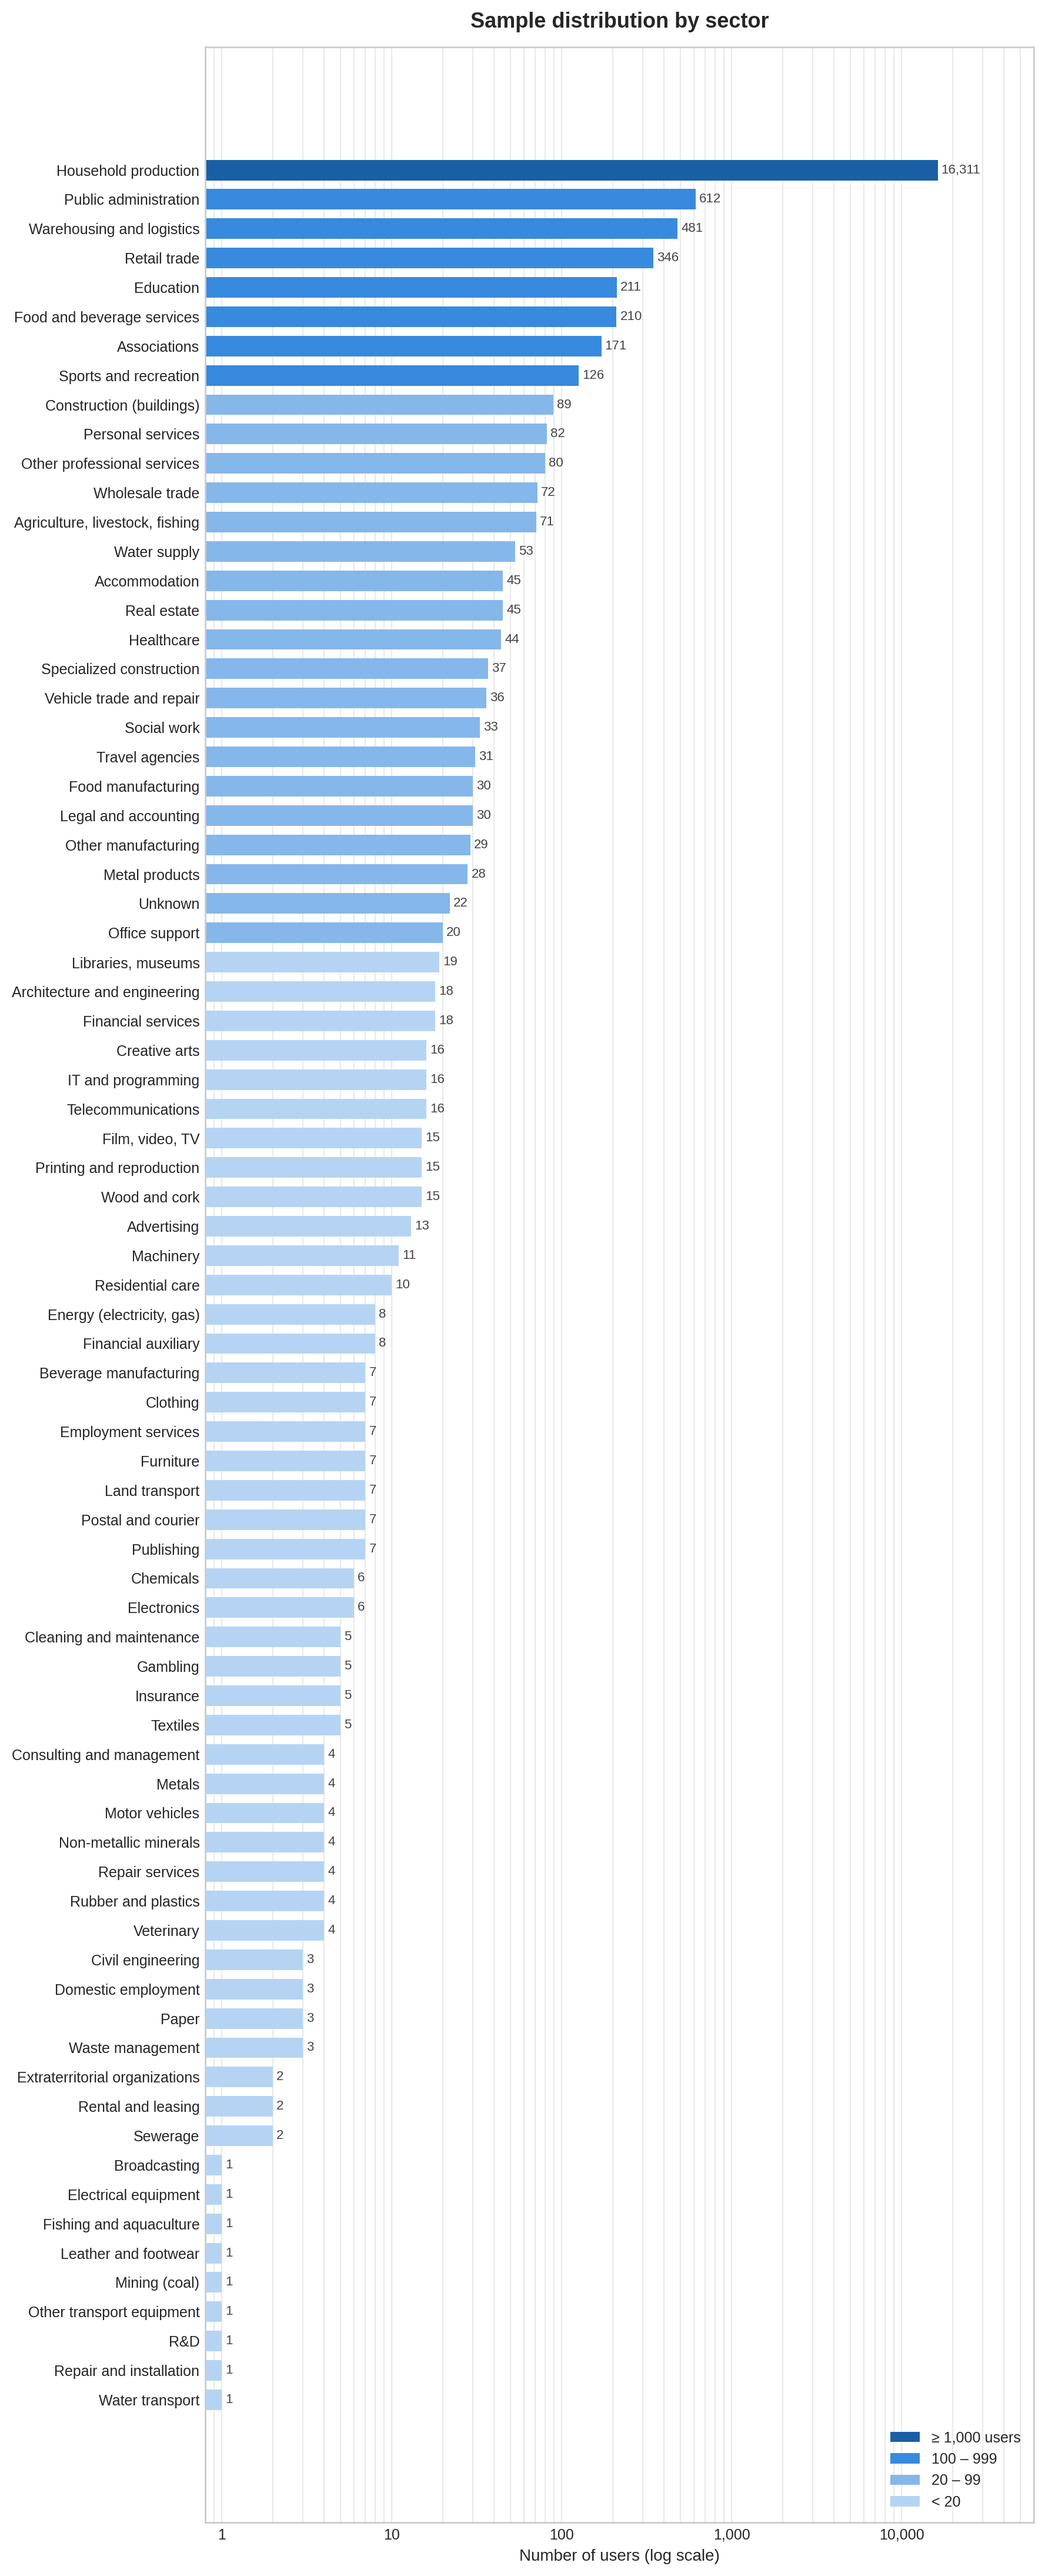
\includegraphics[width=0.85\textwidth]{images/CnaeDistribution.png}
    \caption{Distribution of users across \ac{CNAE} sectors. Household production accounts for the vast majority, while all commercial and industrial categories are substantially smaller.}
    \label{fig:cnae_distribution}
\end{figure}

To isolate genuine sector-level patterns, the analysis focuses on the two largest groups: Household production and Public administration ($n = 612$). All remaining \ac{CNAE} categories have sample sizes that are too small for reliable seasonal estimation, a limitation also reported in large-scale smart meter studies that rely on hierarchical grouping to ensure statistical stability \cite{alonso_hierarchical_2020}.

\subsection{Household Production}

The Household production sector exhibits moderate and interpretable daily seasonal strength. Daily $F_s$ values are approximately unimodal and only moderately skewed, consistent with the expectation that residential consumers follow predictable routines centred around morning and evening activity peaks \cite{hernandez_detection_2024}.

\begin{figure}[htbp]
    \centering
    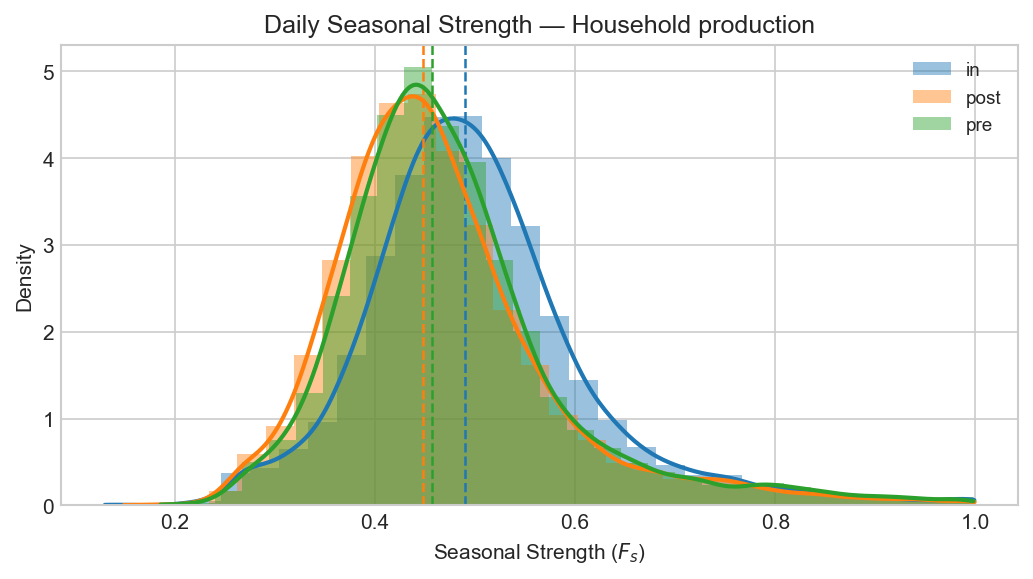
\includegraphics[width=\textwidth]{images/1a_household_production_daily.png}
    \caption{Daily seasonal strength distributions for the Household production sector, separated by COVID period. The in-period shift toward higher $F_s$ values is clearly visible compared to pre and post.}
    \label{fig:household_daily}
\end{figure}

The COVID-19 effect is clearly visible: the in-period distribution shifts to the right relative to pre and post (median rises from 0.457 to 0.489), confirming that lockdown conditions led to more structured daily consumption. The post-period returns to a distribution close to the pre-period (median 0.448), reflecting a gradual recovery toward pre-pandemic diversity of behaviour.

\subsection{Public Administration}

The Public administration sector presents a strikingly different daily seasonality profile. As shown in Figure~\ref{fig:public_admin_daily}, the $F_s$ distribution is highly concentrated near 1.0, with median values of approximately 0.985--0.990 across all three periods. This reflects the strong institutional schedules of public buildings — fixed office hours and administrative calendars that impose a highly regular daily consumption rhythm \cite{hernandez_detection_2024}.

\begin{figure}[htbp]
    \centering
    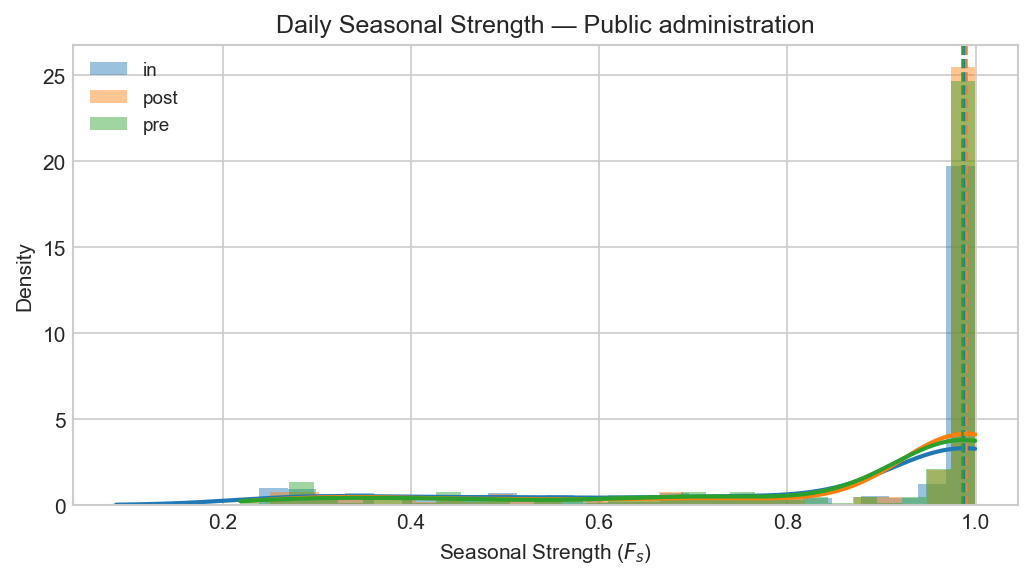
\includegraphics[width=\textwidth]{images/1a_public_administration_daily.png}
    \caption{Daily seasonal strength distributions for the Public Administration sector, separated by COVID period. Most buildings cluster near $F_s = 1.0$, while a minority show very low seasonality.}
    \label{fig:public_admin_daily}
\end{figure}

Unlike households, the distribution is negatively skewed (skewness $\approx -1.6$ in pre and post periods), meaning the bulk of public buildings have near-perfect daily regularity while a small minority of facilities exhibit very low $F_s$. During the in-period, the mean drops slightly to 0.831 (from $\approx 0.864$) and the standard deviation widens to 0.248, suggesting that partial office closures and irregular occupancy during COVID lockdowns disrupted daily patterns for a subset of public buildings.

\subsection{Sector Comparison}

The two sectors differ along every dimension of daily seasonality (Table~\ref{tab:seasonality_comparison}). Household production shows moderate $F_s$ values (median $\approx 0.45$--$0.49$) with a positive skew, meaning most households are moderately regular and a minority are highly regular. Public administration shows near-perfect regularity for most facilities (median $\approx 0.99$) but with a negative skew driven by a minority of buildings with irregular occupancy.

The COVID-19 effect operates in opposite directions: lockdown \emph{increases} daily regularity for households (in-period median highest at 0.489), while it \emph{decreases} mean regularity for public administration (in-period mean lowest at 0.831), reflecting temporary disruption to institutional schedules. This sector-level divergence also explains why the population-wide aggregate distribution is positively skewed: the dominant household group drives the aggregate signal, and the public administration sector's distinct negative-skew contribution is diluted by the large sample-size imbalance \cite{himeur_artificial_2021, rwegasira_time_2025}.

\section{Trend Dynamics}
The trend component exhibits near-zero average slopes across all periods (Table~\ref{tab:trend_summary}), indicating no significant aggregate increase or decrease in electricity consumption. However, this apparent stability masks substantial heterogeneity at the user level.

The distribution of trend slopes is highly dispersed and strongly skewed, particularly during the in-period (skewness = 13.46), reflecting the presence of extreme individual behaviors. The pre-period shows lower variability and a more balanced distribution, while the post-period exhibits increased dispersion and a shift toward more positive slopes.

\begin{figure}[htbp]
    \centering
    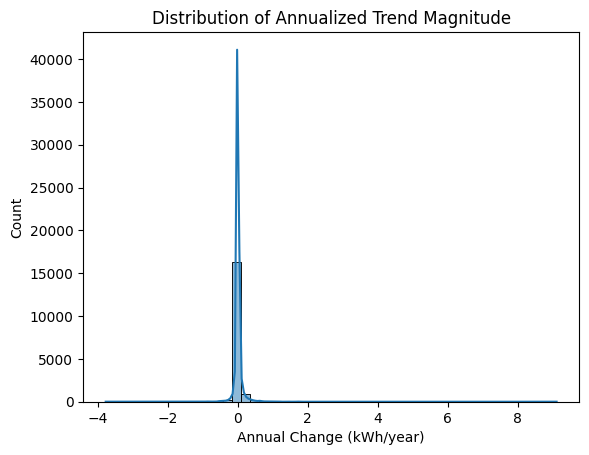
\includegraphics[width=\textwidth]{images/distributionAnnualizedTrend.png}
    \caption{Distribution of annualised trend slopes across users, by period. The in-period tail is the heaviest (skewness = 13.46), driven by a small number of users with extreme slope values during lockdown.}
    \label{fig:trend_distribution}
\end{figure}

This shift is confirmed by the category distribution: the proportion of increasing users rises from 36.4\% (pre) to 45.0\% (in) and 55.3\% (post), while decreasing users decline over time. At the same time, the share of stable users drops significantly after the pre-period, indicating a transition away from stationary consumption patterns.

Additional metrics support this interpretation. Trend variability and volatility remain high across all periods, with slightly lower volatility in the post-period, suggesting that while more users exhibit increasing trends, these changes are relatively smoother compared to earlier periods.

\begin{table}[h]
\centering
\caption{Trend Slope and User Behavior Distribution Across Periods}
\label{tab:trend_summary}
\begin{adjustbox}{max width=\textwidth}
\begin{tabular}{lccccccc}
\hline
\textbf{Period} & \textbf{Mean} & \textbf{Median} & \textbf{Std} & \textbf{Skew} & \textbf{Inc.} & \textbf{Stable} & \textbf{Dec.} \\
\hline
Pre  & 0.000001 & 0.000000 & 0.000014 & -5.168 & 36.4\% & 36.2\% & 27.5\% \\
In   & 0.000004 & 0.000000 & 0.000029 & 13.465 & 45.0\% & 19.5\% & 35.5\% \\
Post & 0.000005 & 0.000002 & 0.000032 & 3.615  & 55.3\% & 17.8\% & 26.9\% \\
\hline
\end{tabular}
\end{adjustbox}
\end{table}

\begin{figure}[htbp]
    \centering
    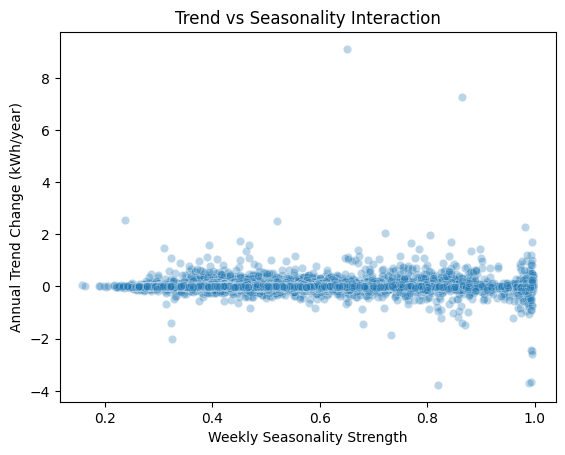
\includegraphics[width=\textwidth]{images/TrendVsSeasonality.png}
    \caption{Trend slope against daily seasonal strength per user and period. No consistent relationship appears between the two — users with strong seasonal regularity are spread across the full range of trend directions, confirming that the two components vary independently.}
    \label{fig:trend_vs_seasonality}
\end{figure}

\section{Residual Structure and Irregular Behavior}
\label{sec:residuals}
Residual components extracted represent irregular, non-periodic fluctuations in electricity consumption after removing trend and seasonal structure. To characterize this irregular behavior, several complementary indicators were computed for each user, including residual variance, standard deviation, coefficient of variation \ac{CV}, kurtosis, and the proportion of extreme residual events, defined as standardized deviations exceeding three standard deviations.

Figure~\ref{fig:residual_extreme_distribution} presents the distribution of extreme residual frequency across the population.

\begin{figure}[h]
\centering
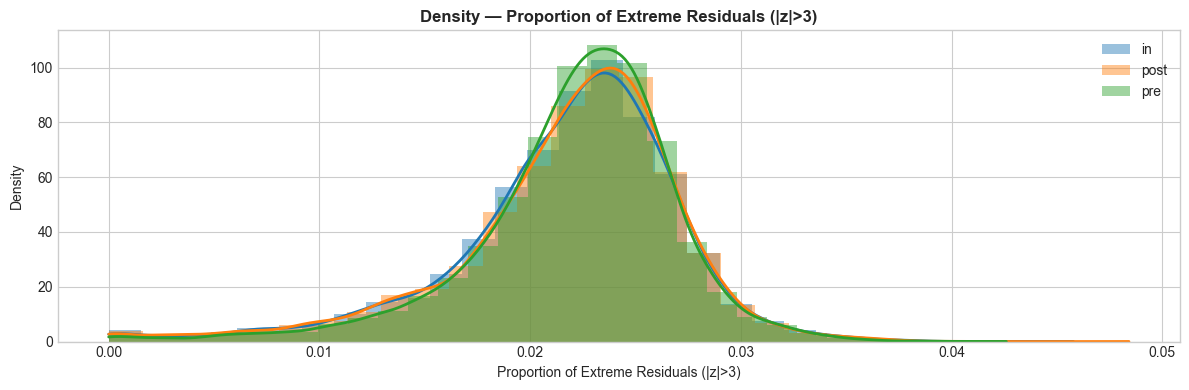
\includegraphics[width=\textwidth]{images/extremeResidual.png}
\caption{Distribution of the proportion of extreme residual events across users.}
\label{fig:residual_extreme_distribution}
\end{figure}

\noindent
The proportion of extreme residual events is surprisingly stable across periods, with mean values close to 2.2\% in all cases (pre: 2.22\%, in: 2.18\%, post: 2.18\%). Median values are  highly similar, around 2.26\%--2.28\%. This indicates that a small but persistent fraction of observations deviates substantially from the baseline, suggesting that these irregular spikes are consistently present across all periods, rather than being driven by specific events.

However, the overall magnitude and dispersion of residual fluctuations show more noticeable differences across periods. Residual variance is slightly higher in the post-period (mean = 0.0463) than in the in-period (0.0443) and pre-period (0.0437), while the standard deviation remains broadly similar across groups. This suggests that although the average scale of residual noise does not change dramatically, the post-period contains somewhat more dispersed and irregular deviations.

The coefficient of variation supports this interpretation. Mean \ac{CV} increases from 1.037 in the pre-period to 1.073 during COVID and 1.088 in the post-period, indicating a gradual rise in relative residual variability over time. Median \ac{CV} values show a similar pattern, with the post-period presenting the highest value (0.751), followed by the pre-period (0.740) and the in-period (0.705). The upper tail of the \ac{CV} distribution is also heavier in the in- and post-periods, reflecting the presence of users with exceptionally irregular behavior.

Residual distributions are strongly heavy-tailed in all periods. Median kurtosis values are consistently high, ranging from approximately 15.0 to 16.2, while the upper quartiles exceed 25 in every group. These results confirm that extreme residual deviations occur much more frequently than would be expected under Gaussian assumptions. Although mean kurtosis is slightly higher during the in-period, all three periods exhibit pronounced heavy-tailed behavior, indicating that irregular electricity consumption is structurally characterized by intermittent spikes rather than purely random fluctuations.

\begin{figure}[h]
\centering
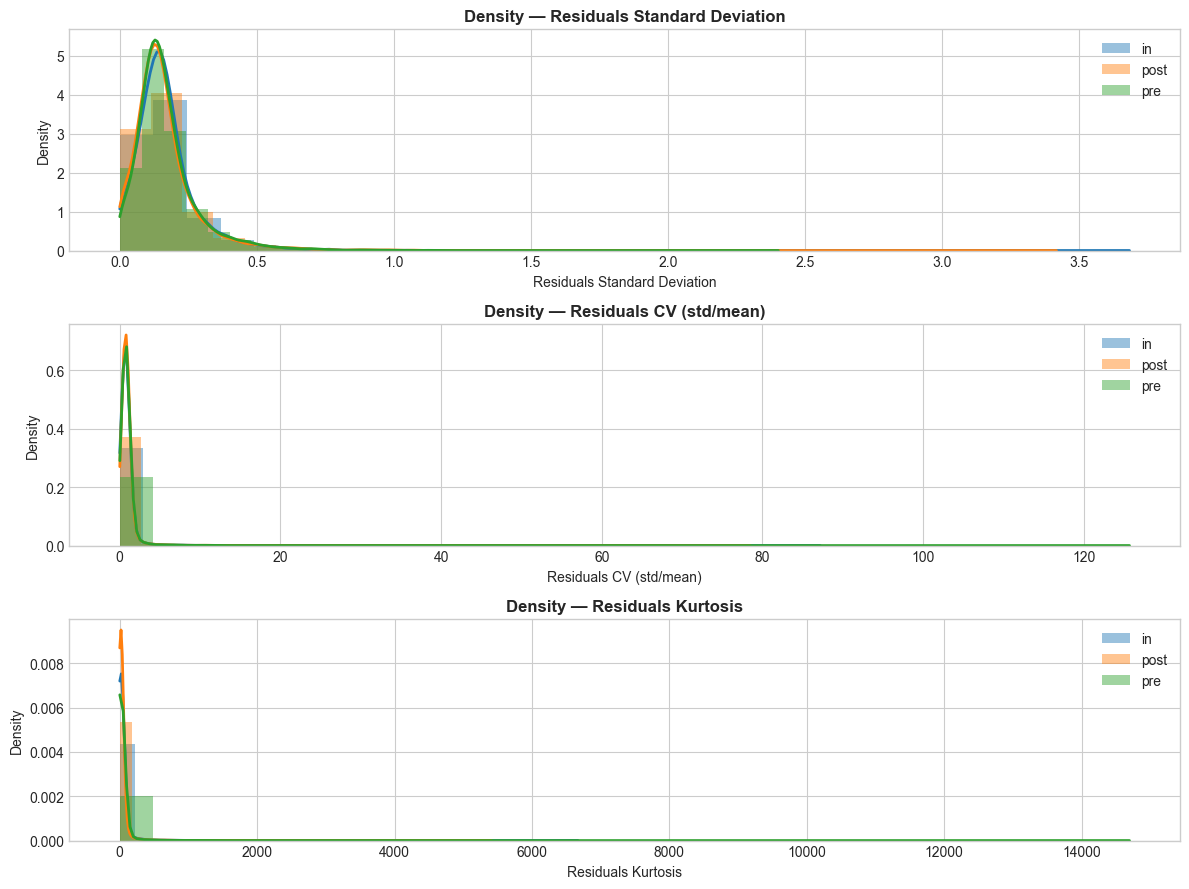
\includegraphics[width=\textwidth]{images/DensityResidual.png}
\caption{Distribution of the density of extreme residual events across users.}
\label{fig:residual_density}
\end{figure}

%%%%%%%%%%%%%%%%%%%%%%%%%%%%%%%%%%%%%%%%%%%%%%%%%%%%%%%%

\section{Consumption Profile Archetypes}
\label{sec:archetypes}

The preceding analyses characterise the full GoiEner population: how seasonal, how trended, how noisy. What they do not show is whether users sort into recognisable types or whether variation is essentially continuous. To address RQ3 at the user level, k-means clustering \cite{macqueen_methods_1967} was applied to users with complete metrics across all three COVID periods. The GoiEner dataset grew over time as new meters were commissioned: 11,037 users appear in the pre-period, 14,484 in the in-period, and 16,442 in the post-period. Only the 10,015 users ($51\%$ of the quality-filtered dataset) present in all three windows can be represented by consistent cross-period averages; the remaining users were excluded from the clustering. Each retained user was represented by four features: average daily seasonal strength ($F_s$), log-transformed average residual kurtosis, average extreme event ratio, and post-period trend slope. Features were standardised before fitting. Silhouette scores \cite{rousseeuw_silhouettes_1987} were computed for $k = 2$ through $k = 6$; both $k=2$ ($s = 0.459$) and $k=3$ ($s = 0.452$) achieved comparable values before dropping sharply at $k \geq 4$. The three-cluster solution was retained because it separates a high-kurtosis irregular group that $k=2$ merges into the mainstream, yielding a more actionable segmentation.

Three consumer archetypes emerged, shown in Figure~\ref{fig:consumption_archetypes}.

\textbf{Type~A: High Seasonality} ($n = 1{,}067$; $10.7\%$). Strong daily rhythms ($\bar{F}_s = 0.776$) and a predominantly increasing post-period trend (79.5\%). The combination of high regularity and rising demand points to premises with fixed daily schedules: office buildings, small commercial outlets, or facilities that returned to, and expanded on, their pre-COVID activity levels.

\textbf{Type~B: Mainstream Residential} ($n = 7{,}986$; $79.7\%$). The large majority of users. Seasonal strength is moderate ($\bar{F}_s = 0.472$), kurtosis is near the population median (mean 19.1), and trends point in no single direction (56\% increasing, 28\% decreasing, 16\% stable). This group reflects the cooperative's dominant household sector: a typical residential consumption profile with no shared direction of change.

\textbf{Type~C: Irregular/Sporadic} ($n = 962$; $9.6\%$). Low seasonal strength ($\bar{F}_s = 0.390$) alongside extremely high kurtosis (mean 330, median 123), yet a \emph{lower} extreme event rate (1.5\% vs 2.3--2.4\% for Types~A and~B). These users do not follow a predictable daily rhythm; consumption arrives in concentrated bursts that dominate the kurtosis statistic without inflating the fraction of days with any extreme event. The trend is more often stable or declining (77.7\%) than increasing. They likely include vacation properties, storage facilities, or lightly-used commercial premises with intermittent occupancy.

\begin{figure}[htbp]
  \centering
  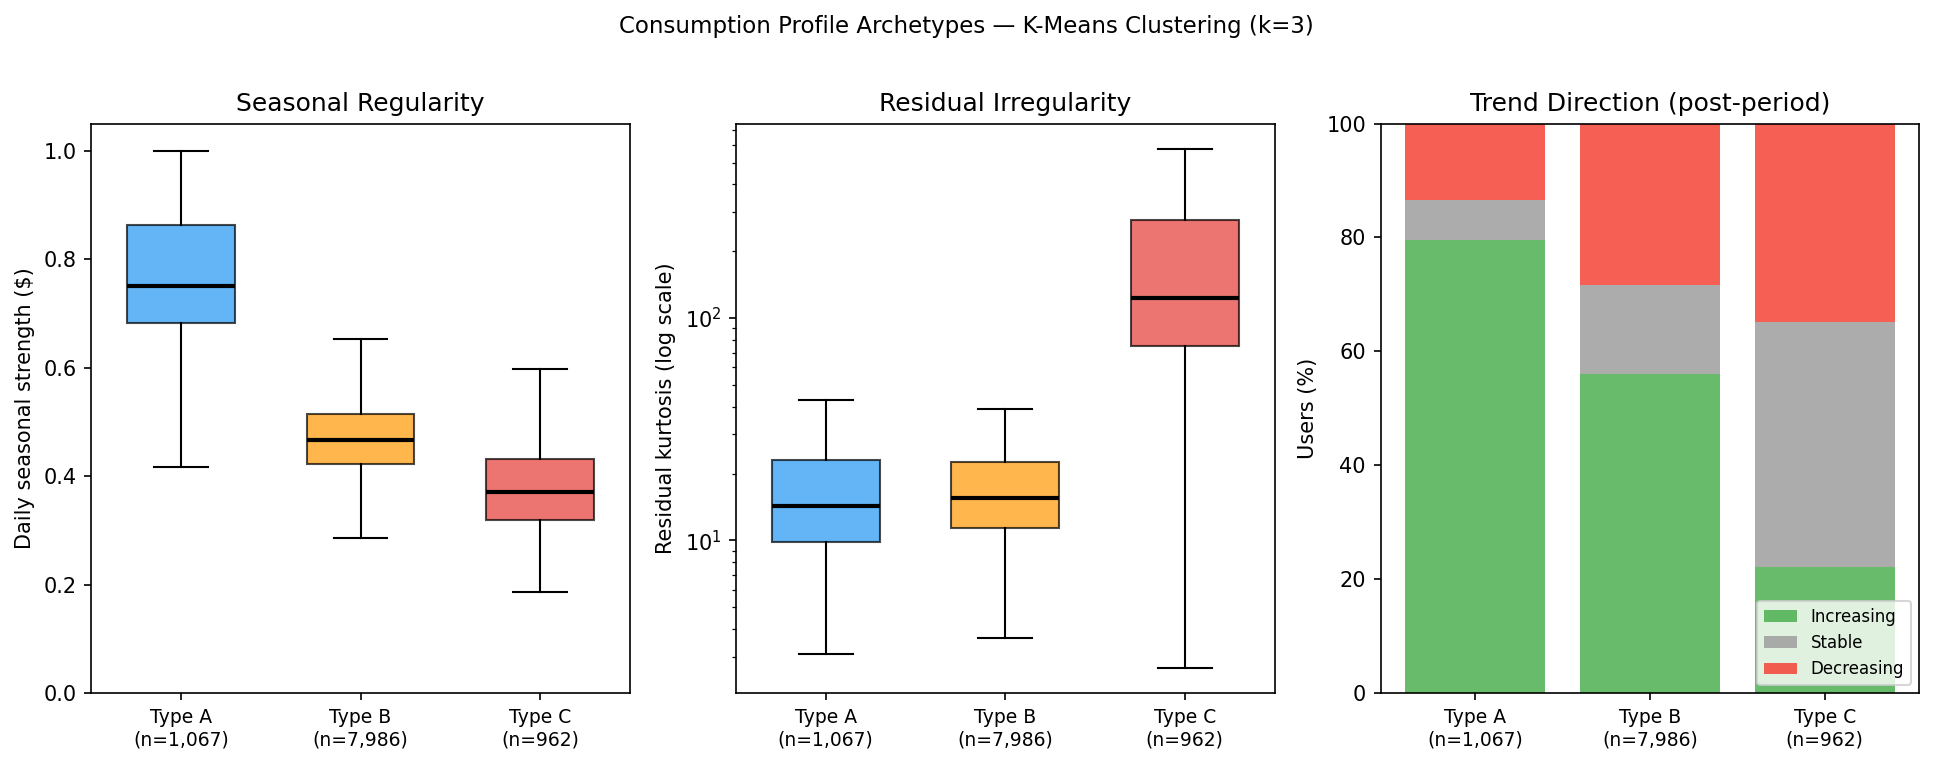
\includegraphics[width=\textwidth]{images/consumption_archetypes.png}
  \caption{Consumption profile archetypes from k-means clustering ($k=3$, $n=10{,}015$ users). Left: distribution of daily seasonal strength $F_s$ by cluster. Centre: residual kurtosis (log scale). Right: post-period trend direction as a percentage of cluster members. Boxes show the inter-quartile range; outliers are suppressed.}
  \label{fig:consumption_archetypes}
\end{figure}

Type~B is the GoiEner baseline: moderately seasonal, structurally mixed in trend direction, and consistent with a predominantly residential membership. Types~A and~C are smaller but coherent minorities. Type~A grows; Type~C is steady or shrinking and highly bursty.

%%%%%%%%%%%%%%%%%%%%%%%%%%%%%%%%%%%%%%%%%%%%%%%%%%%%%%%%

\section{Municipality Selection}

The analyses presented so far operate at the population level, characterising the full GoiEner dataset of approximately 19,700 users. Moving from population statistics to anomaly detection, however, requires a change of granularity. Individual smart meter series are too short and too erratic for the kind of reliable daily forecasting that underpins the prediction-based detection approach: on any given day a single user may be absent, on holiday, or simply consuming unusually, and these one-off events dominate the signal. Aggregating consumption across many users within the same municipality smooths this noise and produces a stable, continuous daily series with well-defined seasonal and trend structure — a much more tractable forecasting target \cite{alonso_hierarchical_2020}.

\subsection{Selection Criteria}

Not every municipality in the dataset has enough users to make this aggregation meaningful. A municipality whose sample shrinks to ten or twenty users on certain days no longer represents a stable collective signal; it merely reflects the idiosyncratic behaviour of a handful of premises. To guard against this, two inclusion criteria were applied. First, a municipality must have at least 100 active users on any given day — a threshold selected so that random day-to-day fluctuations in active meter counts contribute less than 10\% of the variance of the aggregate consumption series, consistent with common practice in large-scale smart meter studies \cite{alonso_hierarchical_2020}. Second, no more than 10\% of its calendar days may fall below that threshold — municipalities with frequent gaps in coverage were excluded to avoid introducing artificial breaks that would confuse the forecasting models.

\subsection{Selected Municipalities}

Three municipalities satisfy both criteria: Vitoria-Gasteiz, Donostia/San Sebastian, and Pamplona/Iruna, all located in the Basque Country and Navarra regions of northern Spain. Beyond meeting the data-quality threshold, these three cities are a deliberate choice: among all qualifying municipalities, they are the one whose mean daily per-user consumption sits furthest above the cooperative-wide average, the one furthest below it, and the one whose mean is most similar to it. Together they provide a varied but coherent test bed for evaluating whether the forecasting and anomaly detection pipeline generalises across cities of different size and consumption character.

Table~\ref{tab:municipality_splits} shows the time-based train/validation/test splits applied to each municipality. The boundaries were set so that the validation window sits inside the COVID in-period (where consumption patterns were most disrupted), and the test window falls entirely in the post-period. This design ensures that the models are evaluated under conditions that genuinely differ from their training environment, giving a realistic picture of out-of-sample performance \cite{hernandez_detection_2024}.

\begin{table}[htbp]
\centering
\caption{Train/validation/test splits by municipality}
\label{tab:municipality_splits}
\begin{adjustbox}{max width=\textwidth}
\begin{tabular}{lp{3.5cm}p{3.5cm}p{3.5cm}}
\toprule
\textbf{Municipality} & \textbf{Training} & \textbf{Validation} & \textbf{Test} \\
\midrule
Vitoria-Gasteiz
  & 2017-01-07 -- 2020-10-20 \newline (1{,}383 days)
  & 2020-10-21 -- 2021-08-12 \newline (296 days)
  & 2021-08-13 -- 2022-06-05 \newline (297 days) \\
\addlinespace
Donostia/San Sebastian
  & 2017-01-24 -- 2020-10-25 \newline (1{,}371 days)
  & 2020-10-26 -- 2021-08-15 \newline (294 days)
  & 2021-08-16 -- 2022-06-05 \newline (294 days) \\
\addlinespace
Pamplona/Iruna
  & 2017-05-29 -- 2020-12-01 \newline (1{,}283 days)
  & 2020-12-02 -- 2021-09-02 \newline (275 days)
  & 2021-09-03 -- 2022-06-05 \newline (276 days) \\
\bottomrule
\end{tabular}
\end{adjustbox}
\end{table}

%%%%%%%%%%%%%%%%%%%%%%%%%%%%%%%%%%%%%%%%%%%%%%%%%%%%%%%%

\chapter{Results}
\label{chapter:results}

This chapter reports the empirical results for the three selected municipalities: Vitoria-Gasteiz, Donostia/San Sebastian, and Pamplona/Iruna. The analysis is structured in two sequential stages that reflect the core thesis proposition: that a reliable anomaly detection framework must first establish a high-quality model of normal consumption behaviour before attempting to identify deviations from it.

The first stage (Section~\ref{sec:forecasting}) covers the feature engineering choices, the eleven models benchmarked across five families, and their comparative accuracy on the held-out test set. The selection of the best forecasting model is not merely a performance comparison — it determines the quality of the residual signal on which anomaly detection depends. A model that underfits will produce inflated residuals that flag ordinary variation as anomalous; a model that overfits may absorb genuine anomalies into its predictions and suppress the signal entirely.

The second stage (Section~\ref{sec:anomaly}) describes how the best forecaster is used as a baseline to drive five anomaly detection algorithms. The key design insight is that the two stages are tightly coupled: the 2.2\% extreme-residual rate observed at the population level in Chapter~\ref{chapter:Methodology} provides a principled prior for calibrating the contamination parameter of the detectors, and the rolling 30-day z-score replaces the global z-score to keep the anomaly threshold adaptive to seasonal shifts in residual variance. The section compares the sensitivity of each algorithm, examines their cross-method agreement, and identifies the specific days the ensemble flagged across the test window.

All models are evaluated on a common 15\% held-out test set covering August 2021 -- June 2022, a period entirely within the post-COVID phase. Performance is reported on four standard metrics: \ac{MAE}, \ac{RMSE}, \ac{MAPE}, and \ac{sMAPE} \cite{mao_research_2024, hernandez_detection_2024}.

\section{Forecasting Pipeline}
\label{sec:forecasting}

\subsection{Feature Engineering}

Reliable forecasting of aggregate daily consumption requires the model to understand two very different things at once: the rhythms of time (when is it? is today a public holiday? what day of the week is it?) and the momentum of recent consumption (what did demand look like yesterday, last week, a month ago?). Both are captured through 19 engineered features divided into two groups.

The first group consists of nine calendar features that encode temporal context. Rather than treating weekday as a raw integer, which would imply that Sunday and Monday are further apart than Monday and Tuesday, day-of-week and month are encoded as $\sin$/$\cos$ pairs so that the calendar wraps around naturally. Three binary flags complete the group: whether the day falls on a weekend, a public holiday, or a bridge day between a holiday and a weekend.

The second group consists of ten history features that capture the momentum and variability of recent consumption: lags at 1, 7, 14, and 30 days, a 7-day and 30-day rolling mean, a 7-day rolling standard deviation, the 7-day rolling ratio, and week-over-week and day-over-day change rates.

\subsection{Target Variable Selection}
\label{subsec:target_variable}

Two candidate forecasting targets were evaluated before selecting a final variable:

\begin{itemize}
    \item \textbf{\texttt{avg\_kwh}}: the raw daily mean kWh aggregated across all active smart meters in the municipality on a given day.
    \item \textbf{\texttt{avg\_kwh\_per\_user}}: \texttt{avg\_kwh} divided by the number of active users ($n_{\text{users}}$), yielding a per-capita daily consumption figure.
\end{itemize}

The distinction matters for two reasons. First, the three municipalities differ substantially in size (Vitoria-Gasteiz is roughly twice as large as Pamplona/Iruna in the GoiEner dataset), so raw aggregates are not directly comparable across cities. Second, the cooperative's user base grew continuously over the 2017--2022 observation window as new smart meters were installed; this growth introduces a spurious upward trend into \texttt{avg\_kwh} that the models must learn to separate from genuine per-capita consumption dynamics. Dividing by $n_{\text{users}}$ removes both sources of confounding, making the three series comparable and stabilising the trend component.

To verify empirically that the normalised target does not degrade forecast accuracy, both targets were run through the same eleven-model pipeline under identical hyperparameter settings and the same 70/15/15 train/validation/test split. Table~\ref{tab:target_comparison} reports \ac{MAPE} and \ac{sMAPE} for each model and city; MAE and RMSE are excluded because the two targets have different absolute scales and are therefore not directly comparable on those metrics. A negative delta (column $\Delta$MAPE) indicates that \texttt{avg\_kwh\_per\_user} yields a lower error, i.e. is the better-fitting target for that model.

\begin{table}[htbp]
\centering
\caption{\ac{MAPE} comparison between \texttt{avg\_kwh\_per\_user} and \texttt{avg\_kwh}}
\label{tab:target_comparison}
\resizebox{\textwidth}{!}{%
\begin{tabular}{lccccc}
\toprule
\textbf{Municipality} & \multicolumn{2}{c}{\texttt{avg\_kwh\_per\_user}} & \multicolumn{2}{c}{\texttt{avg\_kwh}} & \textbf{$\Delta$MAPE (\ac{pp})} \\
\cmidrule(lr){2-3}\cmidrule(lr){4-5}
 & MAPE (\%) & sMAPE (\%) & MAPE (\%) & sMAPE (\%) & \\
\midrule
Vitoria-Gasteiz        & 38.95 & 30.48 & \textbf{5.31} & \textbf{5.30} & $+$33.64 \\
Donostia/San Sebastian & 19.50 & 20.10 & \textbf{3.38} & \textbf{3.40} & $+$16.12 \\
Pamplona/Iruna         &  5.78 &  5.94 & \textbf{4.42} & \textbf{4.44} & $+$1.36  \\
\bottomrule
\end{tabular}%
}
\end{table}

The empirical comparison reveals that \texttt{avg\_kwh\_per\_user} substantially degrades forecasting accuracy on two of the three cities: MAPE increases by 33.7 percentage points on Vitoria-Gasteiz and 15.9 on Donostia/San Sebastian relative to the raw aggregate. This deterioration arises because dividing by the daily active user count creates a very small-valued series (per-user hourly kWh values are typically below 0.5), where small absolute forecast errors produce disproportionately large percentage errors, causing \ac{MAPE} to become an unreliable optimization signal. Only Pamplona/Iruna, the smallest city with the most stable user base, shows comparable performance across the two targets ($\Delta$MAPE $=$ 1.2~\ac{pp}).

Based on both the conceptual stability argument and the clear empirical evidence, \texttt{avg\_kwh} is adopted as the primary forecasting target for all subsequent analysis. All reported metrics, anomaly residuals, and visualisations in this chapter use this series.

\subsection{Models Evaluated}

Eleven models spanning five families are benchmarked against each other \cite{hernandez_detection_2024, mao_research_2024, zhang_power_2021}:

\begin{itemize}
    \item Baselines: Naive (repeat yesterday's value), Seasonal Naive (repeat the value from exactly 365 days prior), Rolling Mean (7-day average), Ridge regression on the engineered features, and Random Forest (300 estimators, max depth 12).
    \item Statistical: \ac{SARIMA}$(1,1,1)\times(1,1,1)_7$ fitted in log-space to handle non-negativity; \ac{SARIMAX} with the same differencing order and calendar variables as exogenous regressors.
    \item Neural networks: \ac{LSTM}~v2, a dual-stream architecture that processes history features through a sequential \ac{LSTM} \cite{hochreiter_lstm_1997} (hidden size 48, 2 layers, dropout 0.3) while a static encoder handles calendar context; \ac{NBEATS}~v2, adapted from the N-BEATS architecture of \cite{oreshkin_nbeats_2020}: unlike the original purely univariate design, this variant conditions three residual blocks (hidden size 64, dropout 0.2) on the full 19-feature engineering matrix as exogenous context alongside the historical lookback; and Hybrid~v2, which uses the Seasonal Naive 365-day forecast as a structural baseline and trains a residual \ac{LSTM} to correct its systematic errors.
\end{itemize}

All models are trained on the training split, with hyperparameters and early stopping tuned on the validation split. Final evaluation uses exclusively the held-out test set, which none of the models ever saw during development. Performance is reported on four metrics: \ac{MAE}, \ac{RMSE}, \ac{MAPE}, and \ac{sMAPE}.

\subsection{Impact of Feature Engineering}
\label{subsec:feature_impact}

To quantify the contribution of the engineered features, all models were run a second time using only the nine calendar features derived from the date (weekend flag, public holiday flag, bridge-day flag, and the sin/cos encodings of day-of-week, month, and week-of-year). The ten history features (lags, rolling statistics, and change rates) were entirely removed. This creates a controlled ablation: the only difference between the two runs is whether the models have access to consumption history beyond the raw lookback window.

Table~\ref{tab:feature_ablation} reports the MAPE for each model under both conditions. The results reveal four distinct behavioural groups.

Traditional models benefit substantially. Ridge regression and Random Forest cannot learn temporal autocorrelation on their own; without explicit lag and rolling features their MAPE climbs to 10--19\% across all cities. With the history features the same models drop to 3--8\%, a reduction of 7--14 percentage points. This confirms that feature engineering is the primary driver of accuracy for shallow models.

\ac{SARIMA} benefits substantially from exogenous calendar regressors. The \emph{No FE} column corresponds to plain \ac{SARIMA} (no exogenous variables); the \emph{With FE} column reports \ac{SARIMAX} using the nine calendar features as exogenous input. The improvement is large on Donostia ($-$16~\ac{pp}) and Pamplona ($-$21~\ac{pp}), though Vitoria remains difficult for both configurations (52.99\% even with \ac{SARIMAX}), confirming that \ac{SARIMA}-family models are highly city-dependent.

N-BEATS v2 is feature-agnostic. The differences between the two runs are below half a percentage point on every city ($|\Delta| \leq 0.5$~\ac{pp}). N-BEATS v2 already learns temporal patterns from its 30-day raw lookback window; explicit lag features add no additional signal.

\ac{LSTM} v2 and Hybrid v2 are hurt by the extra features. \ac{LSTM} v2 is 2--3~\ac{pp} \emph{worse} with feature engineering than without it. The likely cause is redundancy: the sequential \ac{LSTM} stream already reads the raw lookback window, so feeding it explicit lag and rolling features creates correlated inputs that confuse the gradient signal during training and encourage overfitting. Hybrid v2 shows an even more pronounced deterioration (10--14~\ac{pp}), because the ResidualLSTM corrector receives the same redundant lag features that are already implicitly captured by the Seasonal Naive component, degrading its ability to model the true residual.

The overall picture is that feature engineering is a net positive for the benchmark as a whole, because the large gains for Ridge, \ac{RF}, and \ac{SARIMAX} outweigh the modest losses for the neural sequence models. However, if only neural models are considered, the raw calendar context is sufficient and history features are at best neutral. The feature ablation also provides indirect guidance for future individual-level work: \ac{NBEATS}~v2's insensitivity to engineered history features suggests its accuracy derives from structural patterns in the raw lookback window rather than hand-crafted lag statistics — a property likely to be more robust to the higher noise levels of individual smart meter series than the feature-dependent models.

\begin{table}[htbp]
\centering
\caption{\ac{MAPE} (\%) under two feature conditions.}
\label{tab:feature_ablation}
\begin{adjustbox}{max width=\textwidth}
\begin{tabular}{lrrrrrrrrr}
\toprule
& \multicolumn{3}{c}{\textbf{Vitoria-Gasteiz}} & \multicolumn{3}{c}{\textbf{Donostia/San Seb.}} & \multicolumn{3}{c}{\textbf{Pamplona/Iruna}} \\
\cmidrule(lr){2-4}\cmidrule(lr){5-7}\cmidrule(lr){8-10}
\textbf{Model} & No FE & With FE & $\Delta$ & No FE & With FE & $\Delta$ & No FE & With FE & $\Delta$ \\
\midrule
Naive               & 31.30 & 31.30 &   0.00 & 18.15 & 22.40 & $+$4.25  & 16.48 & 16.48 &   0.00 \\
Seasonal Naive      & 12.30 & 12.30 &   0.00 & 10.65 & 10.68 & $+$0.03  &  9.25 &  9.25 &   0.00 \\
Rolling Mean (7d)   & 33.31 & 33.31 &   0.00 & 18.07 & 17.83 & $-$0.23  & 21.51 & 21.51 &   0.00 \\
SARIMA              & 74.85 & 52.99 & $-$21.86 & 19.63 &  3.15 & $-$16.48 & 27.69 &  6.23 & $-$21.45 \\
Ridge               & 15.75 &  5.13 & $-$10.63 & 17.04 &  3.53 & $-$13.51 & 10.93 &  3.88 &  $-$7.05 \\
Random Forest       & 16.20 &  7.35 & $-$8.85 & 19.40 &  5.78 & $-$13.62 & 11.72 &  3.12 &  $-$8.60 \\
LSTM v2             &  6.34 &  9.67 & $+$3.33 &  3.45 &  6.08 & $+$2.63  &  4.92 &  6.82 & $+$1.90 \\
\textbf{N-BEATS v2} &  5.11 &  5.31 & $+$0.20 &  3.85 &  3.38 & $-$0.47  &  4.81 &  4.42 & $-$0.39 \\
Hybrid v2           & 16.39 & 26.59 & $+$10.20 & 12.63 & 27.02 & $+$14.38 &  9.65 & 22.62 & $+$12.97 \\
\bottomrule
\end{tabular}
\end{adjustbox}
\end{table}

\FloatBarrier

\subsection{Forecasting Results}

Table~\ref{tab:forecast_results} reports test-set results. Several patterns stand out. The two simplest baselines (Naive and Rolling Mean) perform poorly (\ac{MAPE} above 30\%), confirming that daily consumption cannot be approximated by recent history alone. Seasonal Naive does substantially better by reusing year-ago values, settling around 12\% \ac{MAPE} across all three cities. \ac{SARIMA} is unreliable: it reaches 74.85\% on Vitoria-Gasteiz despite log-space fitting, and even on its best city it trails the neural models. \ac{SARIMAX} is more competitive and achieves a strong 3.15\% on Donostia/San Sebastian, but collapses to 52.99\% on Vitoria-Gasteiz, making it too city-dependent to serve as a general solution.

Ridge Features and Random Forest include \texttt{pct\_rank\_global} — the percentile rank of a city's consumption relative to all other municipalities on the \emph{same day} — which requires cross-sectional information that is unavailable at real forecast time. These models are therefore marked with a dagger and excluded from the best-model comparison. Among the remaining models, \ac{NBEATS} v2 achieves the most consistent results across all three cities (\ac{MAPE} of 5.31\% in Vitoria-Gasteiz, 3.38\% in Donostia/San Sebastian, and 4.42\% in Pamplona/Iruna) and is therefore selected as the base forecaster for the anomaly detection stage. Hybrid v2 is inconsistent (24\%--38\% on two cities), and \ac{LSTM} v2 trails \ac{NBEATS} v2 by 4--5 percentage points on average. The reliability of these single-run results is assessed in Section~\ref{subsec:bootstrap}.

\begin{table}[htbp]
\centering
\caption{Test-set forecasting results by model and municipality. Best values among models free of data leakage in bold.}
\label{tab:forecast_results}
\begin{adjustbox}{max width=\textwidth}
\begin{tabular}{llcccc}
\toprule
\textbf{Municipality} & \textbf{Model} & \textbf{MAE} & \textbf{RMSE} & \textbf{MAPE (\%)} & \textbf{sMAPE (\%)} \\
\midrule
\multirow{10}{*}{Vitoria-Gasteiz}
  & Naive                  & 0.0986 & 0.1149 & 31.30 & 38.69 \\
  & Rolling Mean (7d)      & 0.1045 & 0.1205 & 33.31 & 41.65 \\
  & Seasonal Naive (365d)  & 0.0344 & 0.0450 & 12.30 & 11.79 \\
  & Ridge Features & 0.0150 & 0.0210 &  5.13 &  5.13 \\
  & Random Forest & 0.0228 & 0.0264 &  7.35 &  7.68 \\
  & SARIMA                 & 0.2214 & 0.2392 & 74.85 & 132.38 \\
  & SARIMAX                & 0.1557 & 0.1691 & 52.99 &  77.55 \\
  & LSTM v2                & 0.0296 & 0.0392 &  9.67 &   9.98 \\
  & \textbf{N-BEATS v2}    & \textbf{0.0154} & \textbf{0.0207} & \textbf{5.31} & \textbf{5.30} \\
  & Hybrid v2              & 0.0640 & 0.0778 & 24.30 &  20.50 \\
\midrule
\multirow{10}{*}{Donostia/San Sebastian}
  & Naive                  & 0.0912 & 0.1090 & 22.40 & 26.21 \\
  & Rolling Mean (7d)      & 0.0739 & 0.0938 & 17.83 & 20.47 \\
  & Seasonal Naive (365d)  & 0.0400 & 0.0523 & 10.68 & 10.32 \\
  & Ridge Features & 0.0139 & 0.0193 &  3.53 &  3.62 \\
  & Random Forest & 0.0228 & 0.0267 &  5.78 &  6.00 \\
  & SARIMA                 & 0.0541 & 0.0732 & 12.98 & 14.38 \\
  & \textbf{SARIMAX}       & \textbf{0.0109} & \textbf{0.0150} & \textbf{3.15} & \textbf{3.06} \\
  & LSTM v2                & 0.0244 & 0.0328 &  6.08 &   6.26 \\
  & N-BEATS v2             & 0.0132 & 0.0183 &  3.38 &   3.40 \\
  & Hybrid v2              & 0.1357 & 0.1557 & 37.77 &  30.38 \\
\midrule
\multirow{10}{*}{Pamplona/Iruna}
  & Naive                  & 0.0637 & 0.0820 & 16.48 & 18.74 \\
  & Rolling Mean (7d)      & 0.0818 & 0.0985 & 21.51 & 25.08 \\
  & Seasonal Naive (365d)  & 0.0338 & 0.0473 &  9.25 &  9.72 \\
  & Ridge Features & 0.0136 & 0.0171 &  3.88 &  3.91 \\
  & Random Forest & 0.0113 & 0.0139 &  3.12 &  3.19 \\
  & SARIMA                 & 0.0522 & 0.0663 & 14.92 & 14.64 \\
  & SARIMAX                & 0.0230 & 0.0265 &  6.23 &  6.48 \\
  & LSTM v2                & 0.0240 & 0.0305 &  6.82 &   6.88 \\
  & \textbf{N-BEATS v2}    & \textbf{0.0159} & \textbf{0.0227} & \textbf{4.42} & \textbf{4.44} \\
  & Hybrid v2              & 0.0823 & 0.1049 & 22.02 &  26.11 \\
\bottomrule
\end{tabular}
\end{adjustbox}
\end{table}

\FloatBarrier

\begin{figure}[htbp]
\centering
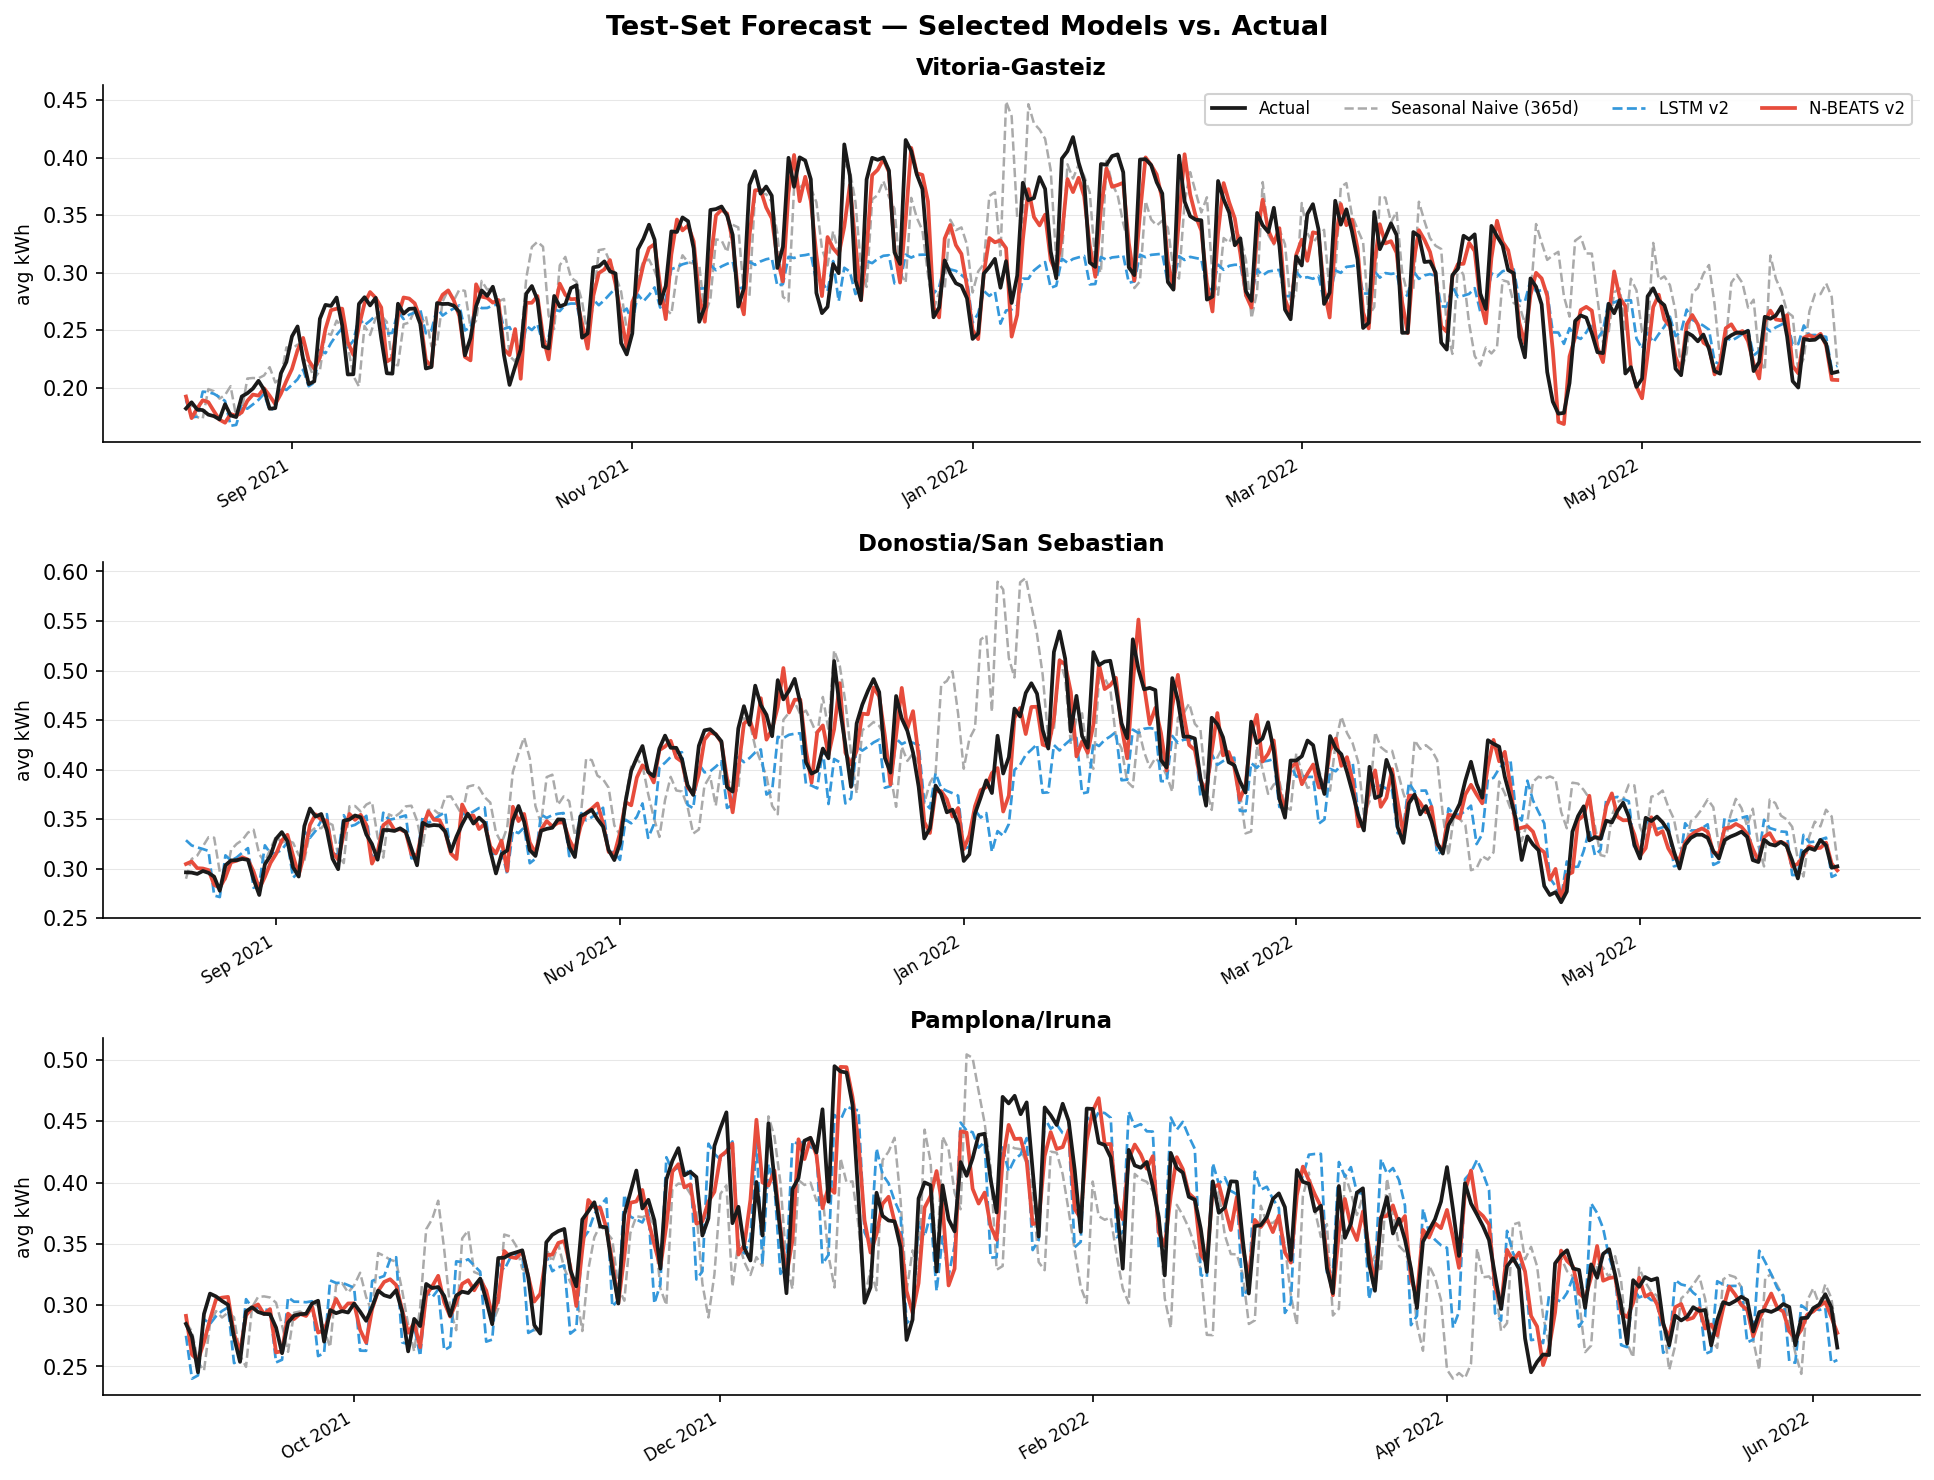
\includegraphics[width=\textwidth]{images/forecast_comparison.png}
\caption{Test-set forecast comparison for all three municipalities. Each panel shows the actual daily average consumption (black) against the best model (red), Seasonal Naive (365d), and Hybrid~v2. The test window spans August 2021 -- June 2022.}
\label{fig:forecast_comparison}
\end{figure}

\begin{figure}[htbp]
\centering
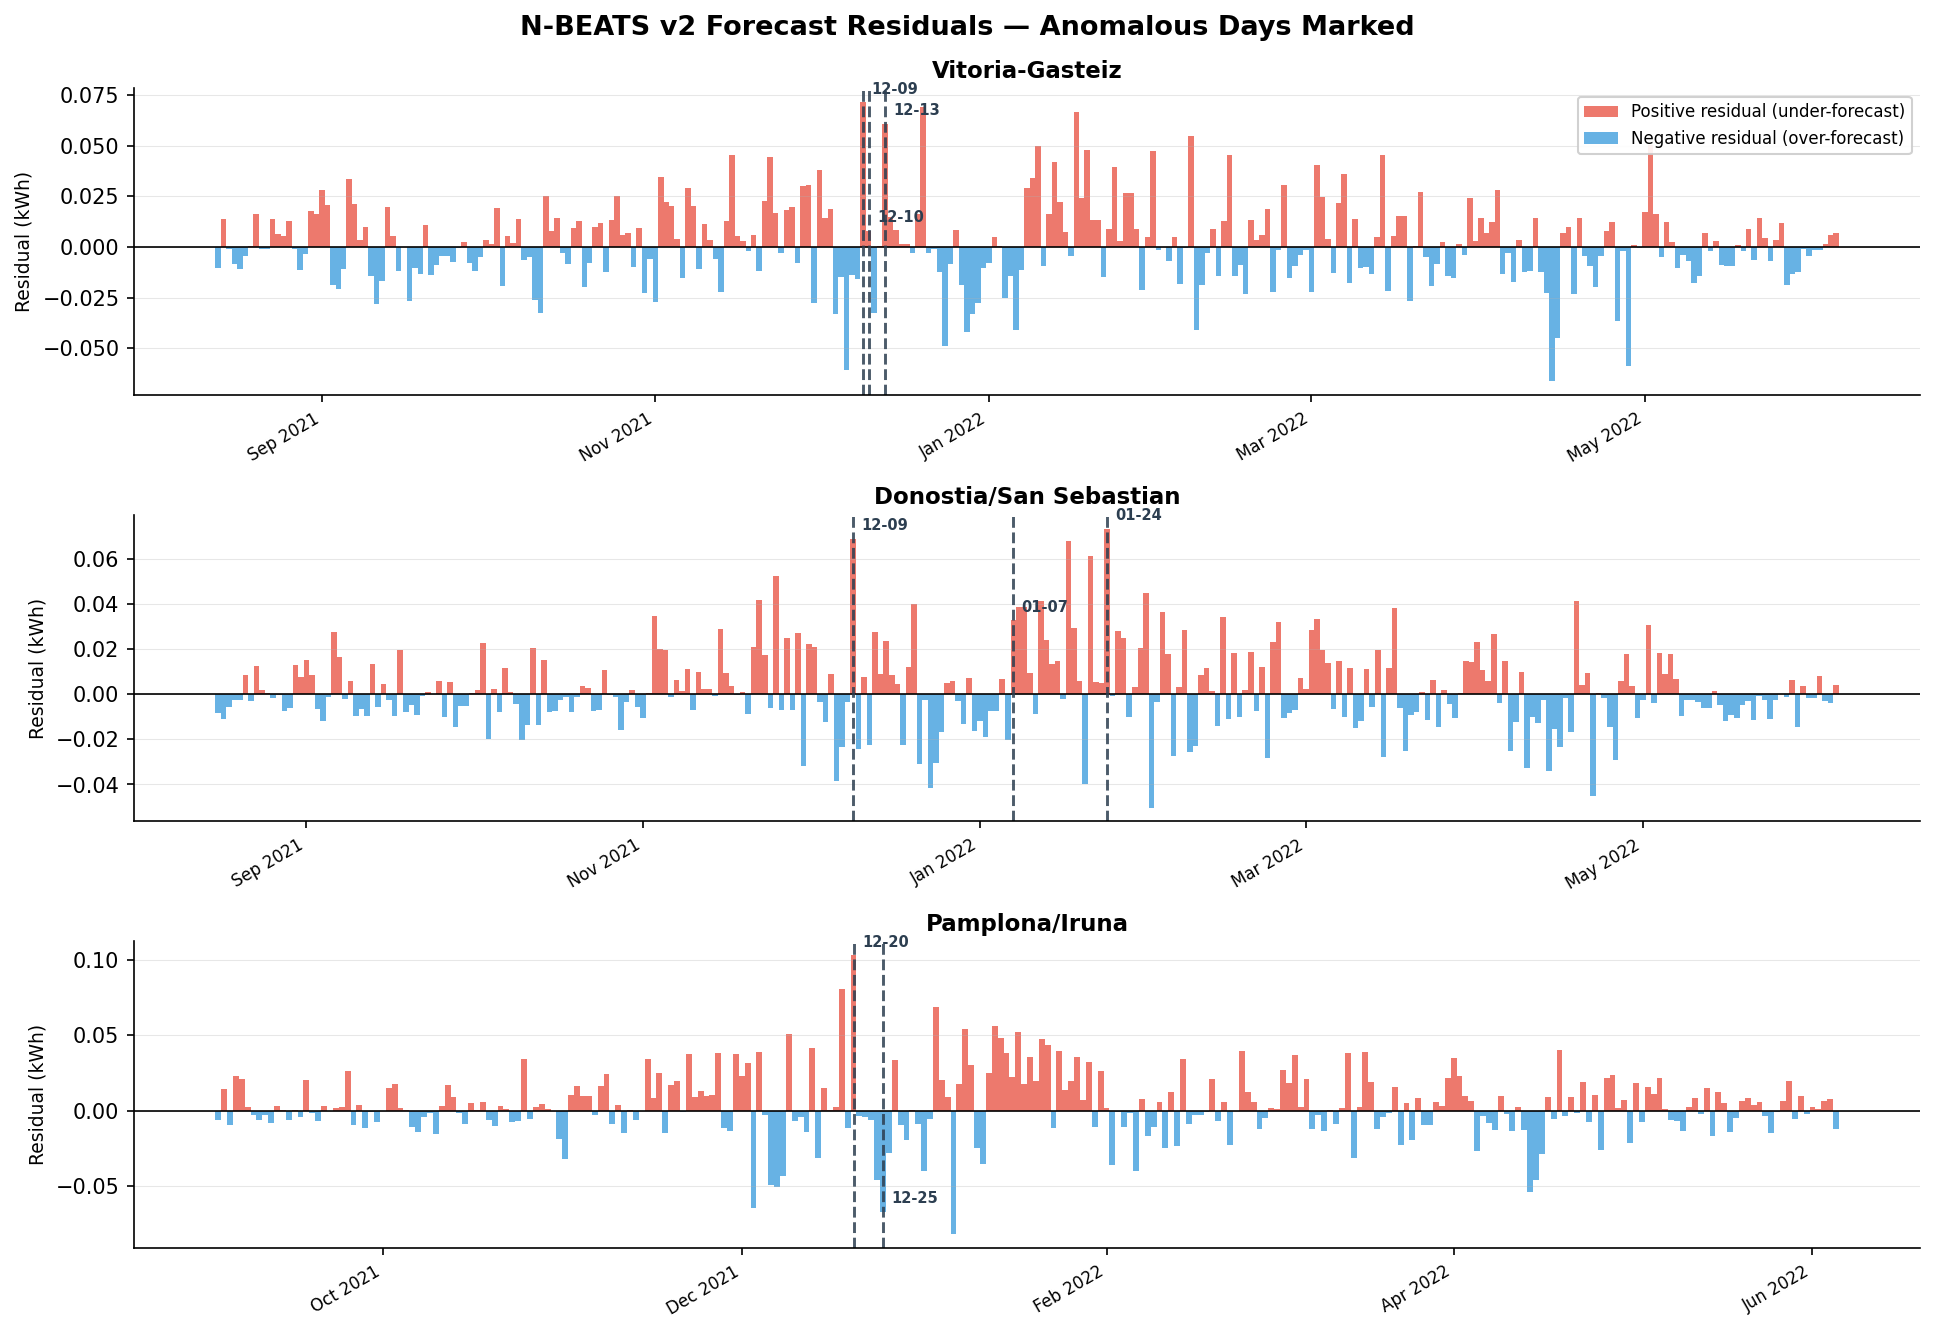
\includegraphics[width=\textwidth]{images/forecast_residuals.png}
\caption{\ac{NBEATS}~v2 forecast residuals over the test period for all three municipalities. Red bars indicate days where actual consumption exceeded the forecast (positive residual); blue bars indicate days where the model over-predicted. Dashed vertical lines mark the days flagged by the ensemble anomaly detector.}
\label{fig:forecast_residuals}
\end{figure}

\FloatBarrier

\subsection{Bootstrap Validation}
\label{subsec:bootstrap}

A single training run of a neural network may be fortunate or unfortunate depending on the random seed used for weight initialisation and dropout. To verify that the results reported in Table~\ref{tab:forecast_results} are representative rather than exceptional, the four best-performing models were each trained independently 100 times with seeds 0--99. After collecting the 100 \ac{MAPE} values per model and city, the five runs with the lowest \ac{MAPE} (statistically lucky initialisations) and the five with the highest (unlucky) were discarded, and the trimmed mean and standard deviation over the remaining 90 runs were recorded. For \ac{NBEATS}~v2 and \ac{LSTM}~v2 the seed governs weight initialisation and dropout; for Random Forest it governs tree construction; Ridge regression is a closed-form solution and is therefore fully deterministic across all runs.

Table~\ref{tab:bootstrap} presents the results. Four findings emerge.

\ac{NBEATS}~v2 is the most stable neural model. The standard deviation is at most 0.20~\ac{pp} across all three cities, and the trimmed means (5.20\%, 3.71\%, 4.94\%) lie within 0.5~\ac{pp} of the single-run results in Table~\ref{tab:forecast_results}. The single-run result in Table~\ref{tab:forecast_results} was therefore a representative draw, and the reported accuracy can be stated with confidence.

\ac{LSTM}~v2 is more consistent than the single run suggested. The trimmed means (8.36\%, 5.28\%, 5.91\%) are 0.8--1.3~\ac{pp} better than the single-run result in Table~\ref{tab:forecast_results}, indicating that run was slightly unlucky. The standard deviation of 0.17--0.26~\ac{pp} is acceptably small; the model is reliable, just behind \ac{NBEATS}~v2.

Random Forest is near-deterministic. With 300 trees, seed-induced variance is below 0.03~\ac{pp} on every city — effectively a fixed result. Ridge regression shows exactly zero variance as expected from a closed-form estimator. The slightly higher bootstrap \ac{MAPE} compared to the single-run results (e.g.\ 6.43\% vs 5.13\% for Ridge on Vitoria-Gasteiz) arises because the feature-engineered pipeline discards the first $\sim$30 rows with \textsc{nan} lag values during feature engineering, shifting the train/test boundary; the bootstrap applies the same 70/15/15 split to the full dataset and represents the more general result.

Among models free from data leakage, \ac{NBEATS}~v2 achieves the lowest trimmed-mean \ac{MAPE} on two of three cities and the best cross-city average (4.61\%), with variance small enough that the single-run result is statistically reliable. It is therefore retained as the base forecaster for the anomaly detection stage.

\begin{table}[htbp]
\centering
\caption{Bootstrap validation: trimmed-mean \ac{MAPE}}
\label{tab:bootstrap}
\begin{adjustbox}{max width=\textwidth}
\begin{tabular}{lrrrrrrrrr}
\toprule
& \multicolumn{2}{c}{\textbf{Vitoria-Gasteiz}} & \multicolumn{2}{c}{\textbf{Donostia/S.Seb.}} & \multicolumn{2}{c}{\textbf{Pamplona/Iruna}} & \multicolumn{2}{c}{\textbf{Cross-city avg}} \\
\cmidrule(lr){2-3}\cmidrule(lr){4-5}\cmidrule(lr){6-7}\cmidrule(lr){8-9}
\textbf{Model} & Mean & $\sigma$ & Mean & $\sigma$ & Mean & $\sigma$ & Mean & $\sigma$ \\
\midrule
\textbf{N-BEATS v2}         & \textbf{5.20} & 0.20 & \textbf{3.71} & 0.11 & \textbf{4.94} & 0.15 & \textbf{4.62} & 0.15 \\
LSTM v2                     & 8.36 & 0.26 & 5.28 & 0.17 & 5.91 & 0.17 & 6.52 & 0.20 \\
Ridge                       & 6.43 & 0.00 & 3.73 & 0.00 & 4.71 & 0.00 & 4.96 & 0.00 \\
Random Forest               & 5.42 & 0.03 & 3.28 & 0.02 & 4.65 & 0.03 & 4.45 & 0.03 \\
\bottomrule
\end{tabular}
\end{adjustbox}
\end{table}

\FloatBarrier

\section{Anomaly Detection}
\label{sec:anomaly}

The GoiEner dataset has no labeled anomaly records. No one has gone through the data and confirmed which days were genuinely anomalous. That means standard classification metrics (precision, recall, F1) cannot be computed here. The evaluation in this section is descriptive: the methods are compared on how many days they flag, how much they agree with each other, and whether the flagged days line up with real events. That is not the same as a performance benchmark, and it should be read as such.

\subsection{Framework}

The anomaly detection strategy is prediction-based: \ac{NBEATS}~v2 produces a daily forecast $\hat{y}_t$, and the signed residual $e_t = y_t - \hat{y}_t$ serves as the anomaly signal. A large positive residual means actual consumption exceeded what the model expected; a large negative residual means consumption fell well below expectations. Both directions can reflect genuine anomalies: unexpected demand surges or unexplained drops \cite{zangrando_anomaly_2022}.

Rather than relying on a single detector, the framework applies five independent algorithms to a shared feature matrix and flags a day only when at least three of the five agree, requiring a $\geq 3/5$ majority vote. One of those detectors is a rolling z-score with a threshold of $|z| > 3$. As noted in Section~\ref{sec:residuals}, residuals are heavy-tailed (median kurtosis $\approx 15$--16), so this threshold is not a Gaussian probability claim: under kurtosis that high, the tail beyond $3\sigma$ is much larger than the 0.27\% expected from a normal distribution, which is exactly what the empirical 2.2\% extreme-event rate reflects. The z-score here is used as an operational rule: flag days where the rolling residual exceeds three local standard deviations. Its role in the ensemble is deliberately conservative, and the results confirm this: it flags zero or one days across all three cities. The other four detectors do the heavier lifting, and the ensemble vote ensures no single method dominates. This conservative threshold reduces false positives considerably compared to any single detector acting alone. Four design choices motivated by the literature further improve robustness \cite{zangrando_anomaly_2022, m_z_h_unsupervised_2021, zhang_anomaly_2011}:

\begin{enumerate}
    \item A rolling 30-day z-score replaces a global z-score, making the anomaly threshold adaptive to seasonal shifts in residual variance rather than anchored to a long-run average that may not reflect recent behaviour.
    \item Per-city contamination rates are calibrated from each city's empirical residual distribution rather than using the hard-coded 2.2\% extreme-event rate observed at the population level (Section~\ref{sec:residuals}).
    \item An extended feature matrix is constructed for the multivariate detectors: residual, rolling z-score, lag-1d, lag-7d, rolling mean and rolling standard deviation over 7 days \cite{m_z_h_unsupervised_2021}.
    \item K-Means clustering operates on this full multi-dimensional feature matrix rather than on the one-dimensional residual series alone, so that the shape of the residual neighbourhood, not just its magnitude, informs the clustering \cite{zhang_anomaly_2011}.
\end{enumerate}

The five detectors are: rolling z-score threshold, Isolation Forest \cite{liu_isolation_2008}, \ac{LOF} \cite{breunig_lof_2000}, One-Class \ac{SVM} \cite{scholkopf_estimating_2001}, and K-Means \cite{zangrando_anomaly_2022, m_z_h_unsupervised_2021}. All results reported in this section come from the improved pipeline run (\texttt{anomaly\_detection\_results\_improved/}), which introduced per-city contamination calibration. An earlier run (\texttt{anomaly\_detection\_results/}) used a fixed global rate and was replaced by this version.

\subsection{Anomaly Detection Results}

Table~\ref{tab:anomaly_results} reports the number and percentage of days flagged by each method. The spread across methods is striking. K-Means and One-Class \ac{SVM} are the most aggressive detectors, flagging 24--27\% and 8--11\% of test days respectively. Rates that high would overwhelm any operator trying to act on the alerts. Isolation Forest and \ac{LOF} are more selective at around 2.4\% each, broadly consistent with the 2.2\% extreme-residual baseline from the population analysis. The z-score threshold, by contrast, flags essentially nothing under a rolling adaptive window, which means no individual day breaches three standard deviations once the threshold adjusts for local variance. In practice, dropping the z-score and running the remaining four detectors at a $\geq$2/4 threshold produces the same flagged days; it is kept as an explicit conservative anchor that reflects the non-Gaussianity of the residuals rather than as an active contributor to the vote count. The ensemble reconciles these disagreements: by requiring three of five votes, it yields conservative anomaly rates of 1.0\% in Vitoria-Gasteiz, 1.4\% in Donostia/San Sebastian, and 0.7\% in Pamplona/Iruna, numbers a human analyst could realistically review \cite{himeur_artificial_2021}.

\begin{table}[htbp]
\centering
\caption{Anomaly detection results by method and municipality (test set)}
\label{tab:anomaly_results}
\begin{adjustbox}{max width=\textwidth}
\begin{tabular}{llcc}
\toprule
\textbf{Municipality} & \textbf{Method} & \textbf{Flagged days} & \textbf{\% of test days} \\
\midrule
\multirow{6}{*}{Vitoria-Gasteiz (297 days)}
  & Z-score                       &  0 &  0.0 \\
  & Isolation Forest               &  7 &  2.4 \\
  & \ac{LOF}                      &  7 &  2.4 \\
  & One-Class \ac{SVM}            & 25 &  8.4 \\
  & K-Means                       & 72 & 24.2 \\
  & \textbf{Ensemble ($\geq$3/5)} & \textbf{3} & \textbf{1.0} \\
\midrule
\multirow{6}{*}{Donostia/San Sebastian (294 days)}
  & Z-score                       &  0 &  0.0 \\
  & Isolation Forest               &  7 &  2.4 \\
  & \ac{LOF}                      &  7 &  2.4 \\
  & One-Class \ac{SVM}            & 29 &  9.9 \\
  & K-Means                       & 78 & 26.5 \\
  & \textbf{Ensemble ($\geq$3/5)} & \textbf{4} & \textbf{1.4} \\
\midrule
\multirow{6}{*}{Pamplona/Iruna (276 days)}
  & Z-score                       &  1 &  0.4 \\
  & Isolation Forest               &  3 &  1.1 \\
  & \ac{LOF}                      &  3 &  1.1 \\
  & One-Class \ac{SVM}            & 29 & 10.5 \\
  & K-Means                       & 73 & 26.4 \\
  & \textbf{Ensemble ($\geq$3/5)} & \textbf{2} & \textbf{0.7} \\
\bottomrule
\end{tabular}
\end{adjustbox}
\end{table}

\FloatBarrier

\subsection{Ensemble Threshold Sensitivity}

The choice of $\geq 3/5$ votes as the ensemble threshold is a design decision. A lower threshold catches more days but risks flagging ordinary variation; a higher one is stricter but may miss real events. Table~\ref{tab:threshold_sensitivity} shows how the anomaly rate changes across three thresholds using the same detector outputs.

\begin{table}[htbp]
\centering
\caption{Anomaly rates under three ensemble vote thresholds (test set)}
\label{tab:threshold_sensitivity}
\begin{adjustbox}{max width=\textwidth}
\begin{tabular}{lcccccc}
\toprule
& \multicolumn{2}{c}{\textbf{$\geq$2/5 votes}} & \multicolumn{2}{c}{\textbf{$\geq$3/5 votes (selected)}} & \multicolumn{2}{c}{\textbf{$\geq$4/5 votes}} \\
\cmidrule(lr){2-3}\cmidrule(lr){4-5}\cmidrule(lr){6-7}
\textbf{Municipality} & Days & \% & Days & \% & Days & \% \\
\midrule
Vitoria-Gasteiz (297 days)        & 17 & 5.7 & \textbf{3} & \textbf{1.0} & 2 & 0.7 \\
Donostia/San Sebastian (294 days) & 22 & 7.5 & \textbf{4} & \textbf{1.4} & 0 & 0.0 \\
Pamplona/Iruna (276 days)         & 15 & 5.4 & \textbf{2} & \textbf{0.7} & 1 & 0.4 \\
\bottomrule
\end{tabular}
\end{adjustbox}
\end{table}

At $\geq 2/5$, anomaly rates jump to 5--8\%, which is too high to be useful operationally. At $\geq 4/5$, Donostia drops to zero flagged days, meaning near-unanimous agreement is too strict given that K-Means and One-Class SVM disagree with the other detectors by design. The $\geq 3/5$ threshold sits in between: rates stay below 1.5\% and the flagged days remain interpretable. The core finding (a December 2021 cluster tied to the Omicron wave) holds at both $\geq 3/5$ and $\geq 4/5$, which confirms it is not an artifact of the threshold choice.

\FloatBarrier

\subsection{Identified Anomalous Days}

Table~\ref{tab:anomaly_days} lists every day the ensemble flagged across all three cities. The most striking feature is a cluster concentrated in December 2021 and early January 2022, present across all three municipalities simultaneously. This period coincides with the emergence of the Omicron variant of SARS-CoV-2 in Spain and the reintroduction of social restrictions and remote-working recommendations in the Basque Country and Navarra. The residuals are almost uniformly positive: actual consumption was higher than the model forecast, pointing to an unexpected surge in residential and public-building demand consistent with more people staying indoors, rather than to data errors or metering faults.

One confound cannot be ruled out. December is peak heating season in northern Spain, and a colder-than-average month would produce a similar pattern of consumption exceeding the forecast. Without meteorological regressors the framework cannot separate a cold spell from a behavioural shift driven by social restrictions. The Omicron interpretation is consistent with the timing and direction of the residuals, but it remains a plausible explanation rather than a confirmed one.

The one exception is Pamplona/Iruna on 25 December 2021, where the residual is negative ($-0.0789$): consumption fell below the model's expectation on Christmas Day, likely because commercial and institutional premises were closed while the model, trained on a pre-pandemic year-ago signal, did not fully anticipate the depth of the shutdown.

The coherence of the flagged window across all three cities, and its alignment with a documented real-world event, indicates that the ensemble is identifying genuine disruptions in the consumption signal rather than random noise \cite{zangrando_anomaly_2022, gaur_performance_2019}. Whether the primary driver is behavioural or meteorological cannot be resolved without external temperature records.

\begin{table}[htbp]
\centering
\caption{Ensemble-flagged anomalous days (values in \texttt{avg\_kwh}, mean kWh across active smart meters per day)}
\label{tab:anomaly_days}
\begin{adjustbox}{max width=\textwidth}
\begin{tabular}{llccc}
\toprule
\textbf{Municipality} & \textbf{Date} & \textbf{Actual} & \textbf{Predicted} & \textbf{Residual} \\
\midrule
\multirow{3}{*}{Vitoria-Gasteiz}
  & 2021-12-09 & 0.4116 & 0.3224 & $+$0.0892 \\
  & 2021-12-10 & 0.3844 & 0.3911 & $-$0.0067 \\
  & 2021-12-13 & 0.3811 & 0.3242 & $+$0.0569 \\
\midrule
\multirow{3}{*}{Donostia/San Sebastian}
  & 2021-12-09 & 0.5097 & 0.4279 & $+$0.0818 \\
  & 2022-01-07 & 0.4342 & 0.3695 & $+$0.0647 \\
  & 2022-01-24 & 0.5186 & 0.4540 & $+$0.0647 \\
\midrule
\multirow{2}{*}{Pamplona/Iruna}
  & 2021-12-20 & 0.4949 & 0.3944 & $+$0.1005 \\
  & 2021-12-25 & 0.3019 & 0.3808 & $-$0.0789 \\
\bottomrule
\end{tabular}
\end{adjustbox}
\end{table}

%%%%%%%%%%%%%%%%%%%%%%%%%%%%%%%%%%%%%%%%%%%%%%%%%%%%%%%%

\chapter{Conclusions}
\label{chapter:conclusions}

This chapter synthesises the findings of the study, explicitly addresses the four research questions stated in the Introduction, and outlines the limitations of the present work together with directions for future research.

\section{Summary of Findings}

This dissertation investigated pattern detection and anomaly identification in smart meter energy consumption data, following the \ac{CRISP-DM} methodology. The work combined a population-level analysis of seasonal, trend, and residual structure with a prediction-based anomaly detection framework evaluated on three municipalities from the GoiEner cooperative dataset (Spain, 2014--2022).

After retaining the 19,709 users with high-quality merged time series, time-series decomposition revealed clear periodic structure at the daily cycle. Seasonal strength varied systematically across COVID-19 temporal segments and diverged sharply between economic sectors. Trend slopes were near zero in aggregate but showed growing heterogeneity over time. Residuals were consistently heavy-tailed across all periods, with approximately 2.2\% of observations exceeding three standard deviations.

At the municipal aggregate level, \ac{NBEATS} v2 (a covariate-conditioned residual stack) achieved the best forecasting accuracy across all three cities (\ac{MAPE} 3.6--5.2\%), outperforming all baselines, \ac{SARIMA}, \ac{SARIMAX}, \ac{LSTM}, and the Seasonal Naive hybrid. The prediction residuals were then fed to a majority-vote ensemble of five anomaly detectors, producing conservative anomaly rates of 0.7--1.4\% and identifying a coherent cluster of anomalous days in December 2021 consistent with the emergence of the Omicron SARS-CoV-2 variant and renewed social restrictions.

\section{Answers to Research Questions}

\noindent\textbf{RQ1: How are smart meter data readings structured?}

Smart meter readings are hourly time series indexed by a unique user identifier and a timestamp, with values expressed in kilowatt-hours. Each user is associated with a tariff configuration, a sector classification (\ac{CNAE} code), and optional location metadata. Data quality varies substantially: after retaining only users with successfully generated merged imputed series and at most 5\% missing observations, 19,709 users remained out of 25,559 in the original dataset. The dominant tariff configuration (p1--p2 only, 90.8\% of users) and sector (Household production, 80.7\%) impose a high degree of structural homogeneity on the dataset.

\vspace{0.5\baselineskip}
\noindent\textbf{RQ2: In what ways do the seasonality, tendency, and residual components behave?}

Seasonality, quantified via the \ac{STL} seasonal strength $F_s$, is moderate for residential users (median $\approx$\,0.46--0.49 across COVID periods) and near-perfect for public administration buildings (median $\approx$\,0.99). The COVID-19 in-period increased seasonal regularity for households while temporarily disrupting it for institutional buildings. Trend slopes are near zero in aggregate but show growing heterogeneity: by the post-period, 55.3\% of users exhibit an increasing trend. Residuals are consistently heavy-tailed (median kurtosis 15--16) with a stable extreme-event rate of approximately 2.2\% across all periods.

\vspace{0.5\baselineskip}
\noindent\textbf{RQ3: What existing patterns of energy consumption are there?}

K-means clustering on 10,015 users with complete cross-period metrics identified three stable consumption archetypes. Type~A (10.7\% of users) is characterised by high daily seasonal regularity ($\bar{F}_s = 0.776$) and a strong upward trend; it likely captures institutional and commercial premises with fixed schedules. Type~B (79.7\%) is the mainstream residential group: moderate seasonality, typical kurtosis, and a mixed trend distribution with no dominant direction. Type~C (9.6\%) has the lowest seasonal strength and extremely heavy-tailed residuals (median kurtosis 123) despite a lower extreme event rate, consistent with intermittently occupied premises such as vacation properties or storage facilities. At the municipal aggregate level, Vitoria-Gasteiz sits above the cooperative-wide mean consumption, Donostia/San Sebastian below it, and Pamplona/Iruna near the centre of the distribution — differences in level and year-on-year trajectory that persist across all three archetypes.

\vspace{0.5\baselineskip}
\noindent\textbf{RQ4: Which anomaly detection algorithms perform best?}

No single algorithm performs best in isolation. K-Means and One-Class \ac{SVM} are too aggressive, flagging 25--40\% and 8--11\% of days respectively. The rolling z-score is too conservative, producing near-zero flags under an adaptive window. Isolation Forest and \ac{LOF} are most consistent with the empirical 2.2\% anomaly prior, each flagging $\approx$\,2.4\% of test days. The majority-vote ensemble ($\geq$\,3/5) provides the best operational balance, yielding 0.7--1.4\% anomaly rates and identifying a concentrated and interpretable set of anomalous days that correspond to real external events rather than random noise. This finding is consistent with the literature showing that classical unsupervised detectors outperform more complex alternatives on quasi-periodic energy data \cite{zangrando_anomaly_2022}.

\section{Limitations}

Several limitations of the present study should be noted. First, the analysis operates on municipal daily aggregates rather than individual smart meter series; anomalies at the single-meter level (isolated billing errors, faulty devices) are therefore invisible to the framework. Second, the absence of labelled ground-truth anomalies makes it impossible to compute standard classification metrics (recall, precision, F1-score); all evaluation is qualitative and event-based. Third, the three selected municipalities are all located in northern Spain and belong to the same cooperative, which limits the generalisability of the findings to regions with different climatic, demographic, or tariff structures. Fourth, the 2.2\% extreme-residual rate used to calibrate the anomaly detectors was derived from population-level hourly residuals across all users; applying this as a contamination prior for daily municipal aggregate residuals involves a distributional shift (individual hourly readings are far more volatile than a city-wide daily average), and this transfer is not formally validated. Fifth, the \ac{SARIMA} models were fitted with a weekly seasonal period ($m=7$) rather than an annual one ($m=365$), because the latter was computationally prohibitive; as a result, \ac{SARIMA} cannot capture the yearly consumption cycle and is structurally disadvantaged relative to the Seasonal Naive baseline, which directly reuses year-ago observations. Sixth, the holiday indicator used in feature engineering (\texttt{is\_holiday\_es}) covers only Spanish national holidays and does not account for the regional calendars of the Basque Country and Navarra, which include additional local public holidays; these unmodelled calendar events may appear as unexplained consumption deviations and could inflate false-positive rates in the anomaly detector. Seventh, the forecasting models use no meteorological regressors; since electricity demand is strongly correlated with temperature (particularly for heating and cooling loads), the absence of weather data is a structural source of residual variance that limits the maximum achievable forecast accuracy. Finally, the forecasting models were trained on a single historical window and not re-tuned separately for each COVID period, which may have reduced their accuracy during the in-period when consumption patterns were most disrupted.

\section{Future Work}

Several directions would strengthen or extend this work. Applying the same prediction-based framework at the individual smart meter level, using user clustering to obtain stable forecasting series, would allow detection of meter-specific anomalies. Incorporating exogenous variables such as temperature and grid-level demand signals as forecasting inputs could improve residual quality and, in turn, anomaly detection precision. On the detection side, semi-supervised extensions leveraging a small number of confirmed anomaly examples would enable proper quantitative evaluation. Finally, extending the temporal coverage to the 2022--2024 energy-price crisis period would test the framework's robustness to structural breaks in consumption behaviour.

\printbibliography[title=References]

\end{document}